\documentclass[slidescentered]{beamer}
\usepackage[english]{babel}
\usepackage[utf8x]{inputenc}
\usepackage[T1]{fontenc}
\usepackage{color}
\usepackage{standalone}
\usepackage{caption}
\usepackage{subcaption}
\usepackage{appendixnumberbeamer}

\setbeamertemplate{items}[circle]
\setbeamertemplate{blocks}[rounded][shadow=true]

%block
\setbeamercolor{block title}{fg=white, bg=purple}
\setbeamercolor{block body}{bg=purple!20}
\setbeamercolor{block title alerted}{fg=white, bg=orange}
\setbeamercolor{block body alerted}{bg=orange!20}
\setbeamercolor{block title example}{fg=white, bg=blue}
\setbeamercolor{block body example}{bg=blue!20}

\usetheme{UniboTesi}

\title[]{ \Large Development of pre and post-processing
steps to a pipeline aimed to identify silent
cerebral infarcts}
\supervisor{Prof. G. Castellani}

\cosupervisor{Prof. D. Remondini \\ Dr. R. Biondi}
\author{Nicolas Biondini}
\date{31/03/2023}
\department{Physics and Astronomy}
\school{Science}
\degree{Master Degree in Physics}

\begin{document}

	\begin{frame}[noframenumbering]
		\titlepage
	\end{frame}
	
	\documentclass[]{standalone}
\setbeamertemplate{itemize item}[circle]

\begin{document}
	\begin{frame}{Sickle Cell Disease and Silent Cerebral Infarcts}{}
	\vspace{-5pt}
	\begin{itemize}
		\item Sickle Cell Disease (SCD) is a group of inherited red blood cell disorders that causes abnormal hemoglobin.
		
		\item Silent Cerebral Infarcts (SCIs) are defined as abnormal MRI of the brain in the setting of a normal neurologic examination.
	\end{itemize}
	\begin{columns}
		\begin{column}{0.25\textwidth}
		\scriptsize
		SCIs appear as:
			\begin{itemize}
			\item \textbf{Hypointense} regions in T1W images.
			\item \textbf{Hyperintense} regions in T2W and FLAIR images.
			\end{itemize}
			
		\end{column}
		
		\begin{column}{0.8\textwidth}
			\begin{figure}[h!]
				\centering
				\begin{subfigure}[b]{0.4\textwidth}
				\centering
					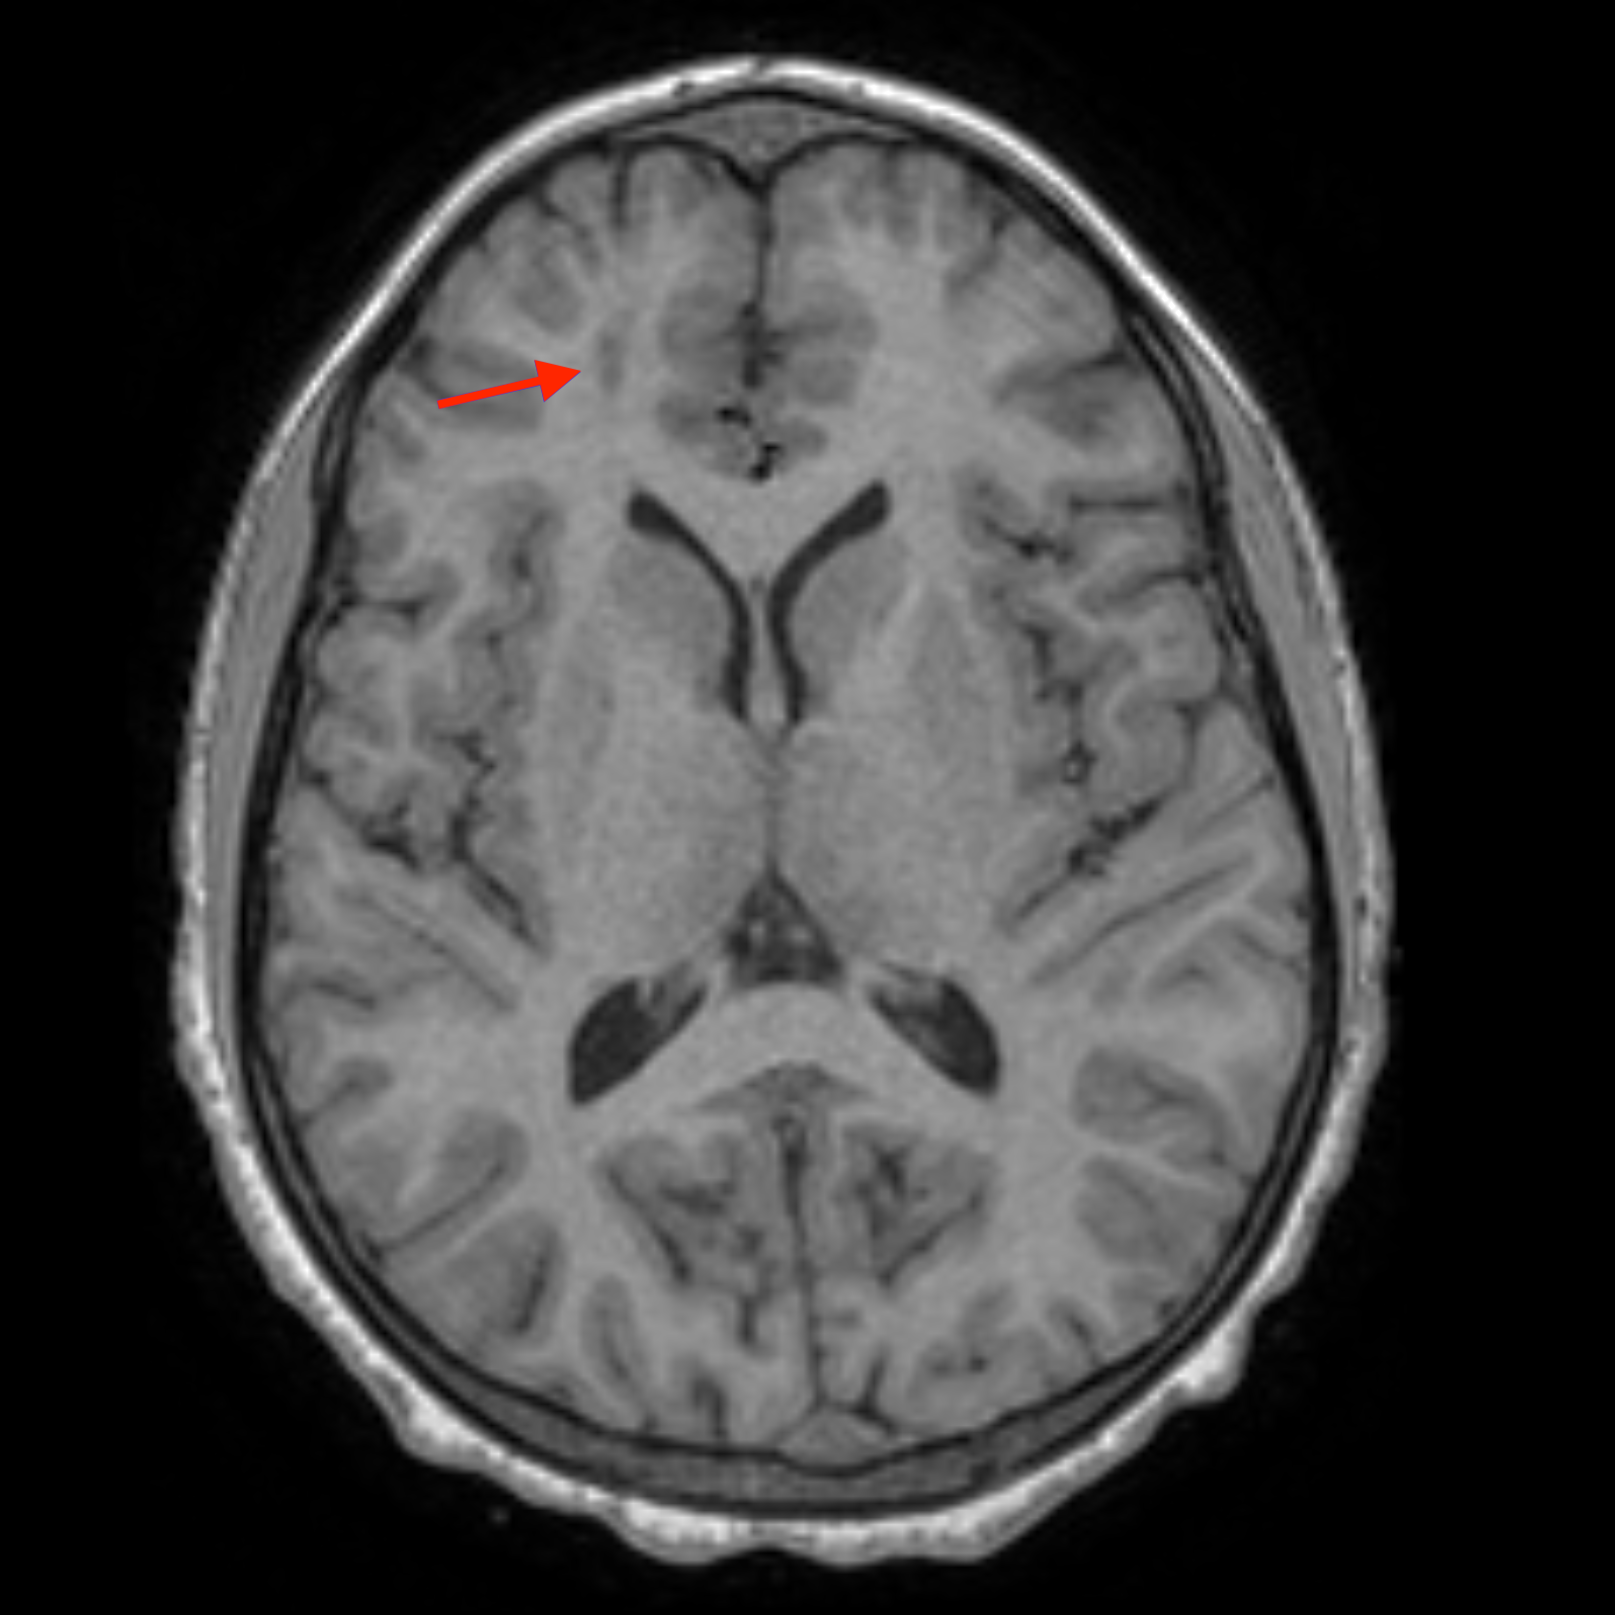
\includegraphics[scale=0.068]{./IMG/Lesion_T1.png}
					\caption*{T1W}
				\end{subfigure} 
				\hspace{20pt}
				\begin{subfigure}[b]{0.4\textwidth}
				\centering
					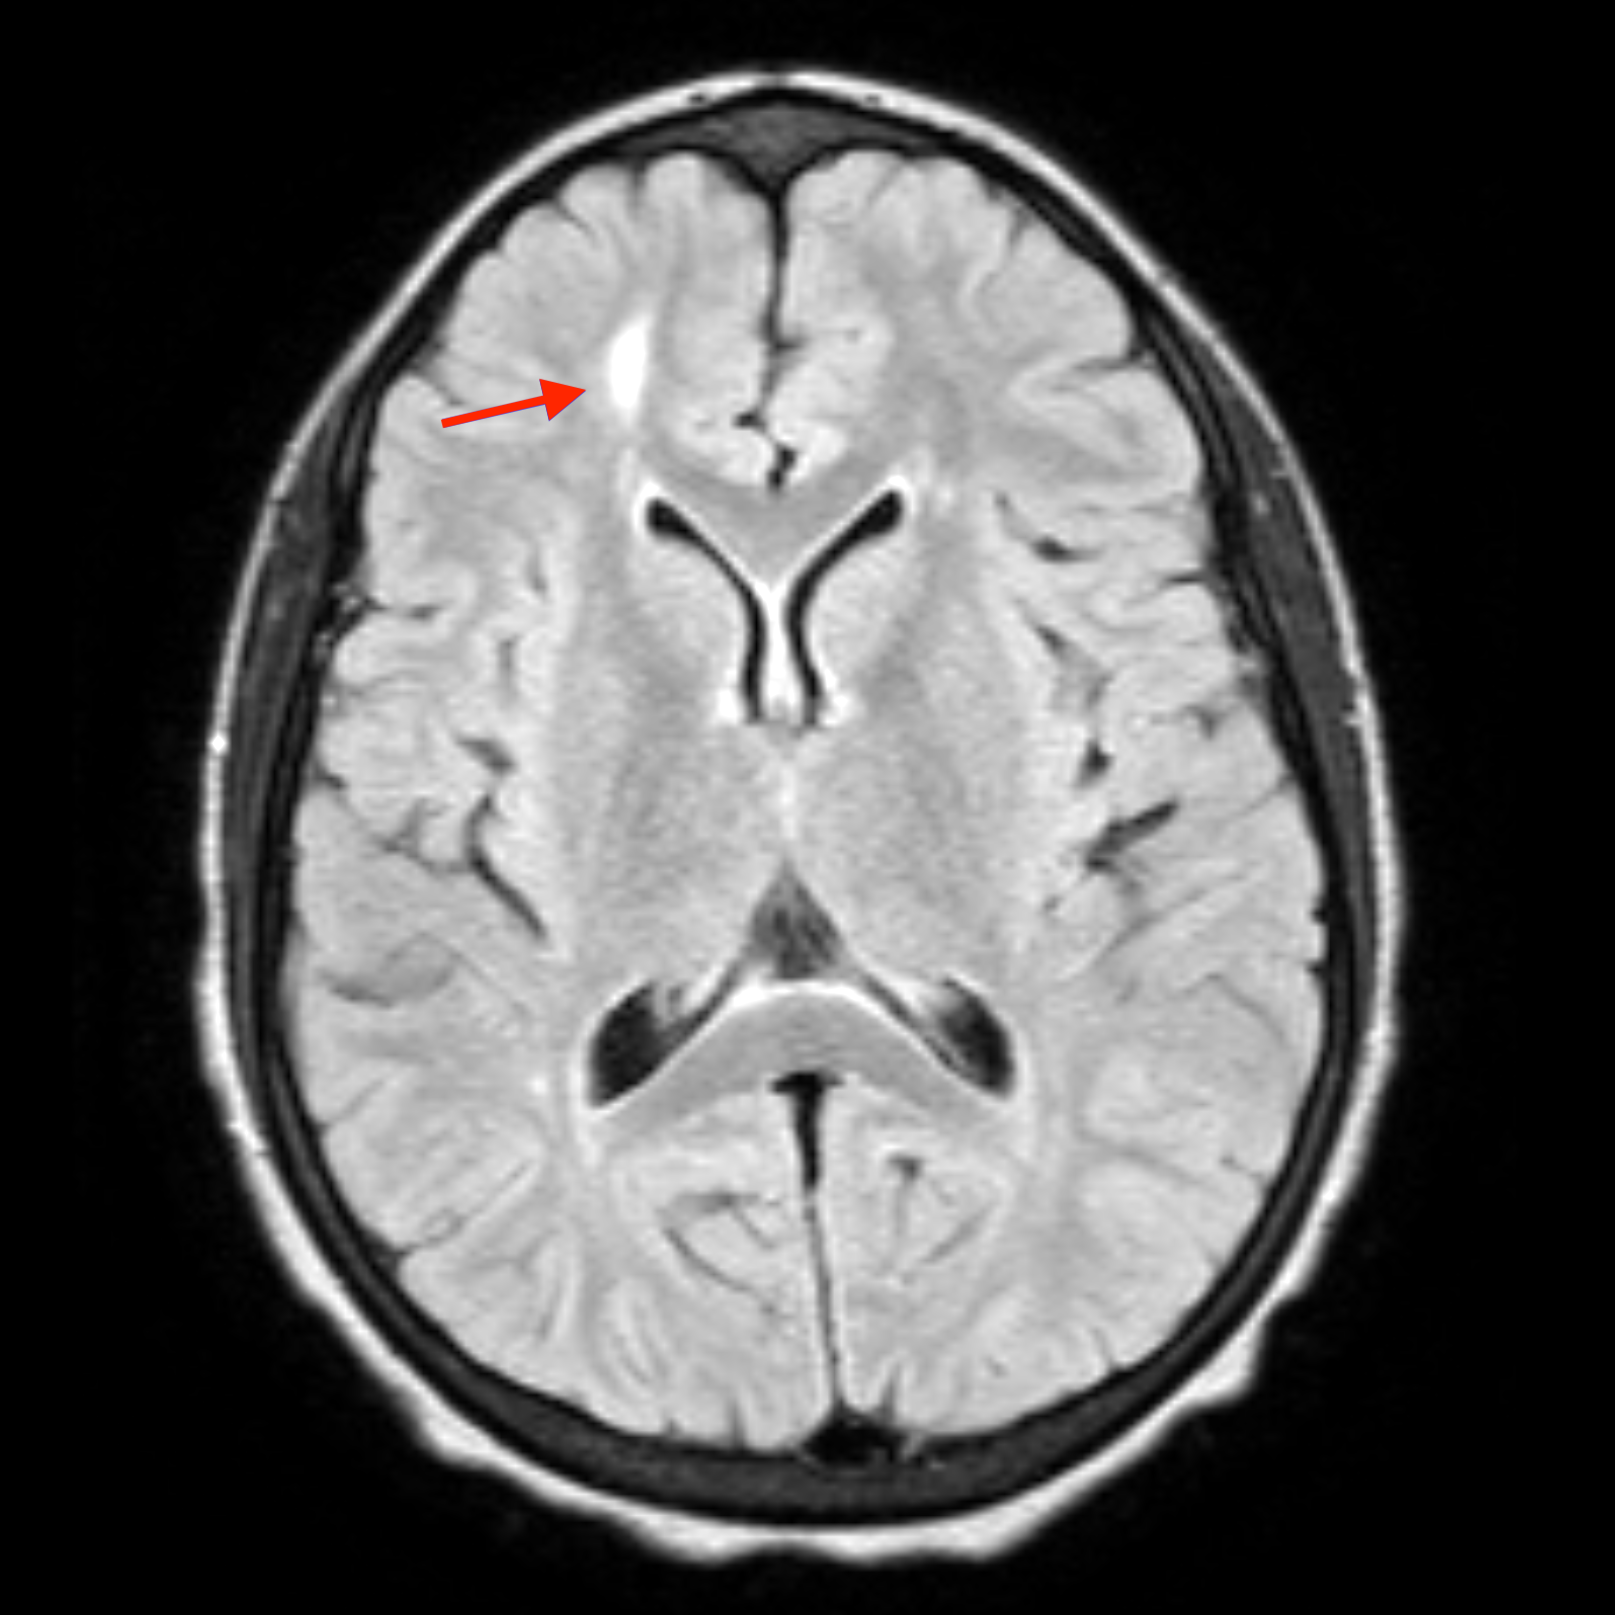
\includegraphics[scale=0.068]{./IMG/Lesion_flair.png}
					\caption*{FLAIR}
				\end{subfigure}
				\hfill
			\end{figure}
		\end{column}
	\end{columns}
	\end{frame}
\end{document}

	
	\documentclass[]{standalone}

\begin{document}
	\begin{frame}{Why Segment SCIs?}{The impact on the quality of life}
	\normalsize
	\vspace{-25pt}
		\begin{exampleblock}{SCIs could lead to:}
			 \begin{itemize}
			 	\item a decrement in general intellectual abilities, 
			 	\item poor academic achievement, 
			 	\item poor working abilities
			 	\item a minor quality of life.
			 \end{itemize}
		\end{exampleblock}
		\vspace{10pt}
		\begin{block}{SCI segmentation is necessary to:}
			\begin{itemize}
				\item understand how SCI negatively affects cognition;
				\item provide a starting point for the identification of potential targets for preventive therapies.
			\end{itemize}
		\end{block}

	\end{frame}
\end{document}

	
	\documentclass[]{standalone}

\begin{document}
	\begin{frame}{How Segment SCIs?}{A Machine and Deep learning approach.}
	\normalsize
	\vspace{-25pt}
		\begin{exampleblock}{Up to now is \textbf{manually} done:}
			\begin{itemize}
				\item made by highly trained and specialized neuroradiologists;
				\item time consuming;
				\item influenced by the experience of the operator.
			\end{itemize}
		\end{exampleblock}
		\vspace{10pt}
		\begin{block}{An \textbf{automatic} pipeline has been proposed:}
			\begin{itemize}
				\item In the contest of the European project \emph{Genomed4All};
				\item Core of the pipeline: pre-trained \textbf{U-Net} ensemble;
				\item \textbf{Pre-processing} step to provided standardized data;
				\item \textbf{Post-processing} step to refine the segmented labels.
			\end{itemize}
		\end{block}	
	\end{frame}
\end{document}

	
	\documentclass[]{standalone}

\begin{document}
	\begin{frame}{Data Set}{Head MRI Scans}
	\vspace{-25pt}
	\begin{columns}
		\begin{column}{0.5\textwidth}
		\begin{exampleblock}{}
		\begin{itemize}
		\footnotesize
			\item 57 MRI \textbf{T1W} and \textbf{FLAIR} head scans;
			\item Acquired from 2009 to 2020;
			\item From three different medical centers in italy;
			\item 51 with SCI evidences, 6 without lesions;
			\item High \textbf{heterogeneity} in both acquisition times and spatial resolution;
			\item Mainly \textbf{underaged} patients;
			\item Manual SCIs segmentation for each scan.
		\end{itemize}
		\end{exampleblock}
		\end{column}
		\begin{column}{0.52\textwidth}
		\begin{block}{}
		\begin{table}[h!]
			\footnotesize
			\setlength{\tabcolsep}{3pt}
			\centering
			\begin{tabular}{|c|cc|cc|}
			\hline
			\textbf{Axis} & \multicolumn{2}{c|}{\textbf{Size (pixel)}} & \multicolumn{2}{c|}{\textbf{Spacing (mm)}} \\
			  & Mean & Std. Dev. & Mean & Std. Dev. \\ \hline
			x & 256  & 0         & 0.85 & 0.12      \\
			y & 256  & 0         & 0.81 & 0.14      \\
			z & 90   & 132       & 4.34 & 1.93      \\ \hline
			\end{tabular}
		\caption*{Spatial Resolution of the images}
		\end{table}
		\vspace{-10pt}
		\end{block}
		\end{column}
	\end{columns}
	\end{frame}
\end{document}

	
	\documentclass[]{standalone}

\begin{document}
	\begin{frame}{Main Pipeline}{U-Net ensemble, Pre-Processing and Post-Processing}
	\vspace{-20pt}
	
	\begin{columns}
		\begin{column}{0.45\textwidth}
			\begin{itemize}
				\item \textbf{Pre-Processing}:
					\begin{itemize}
						\small
						\item Brain Extraction;
					 	\item Gaussian Normalization;
					 	\item Tissue Segmentation;
				 	\end{itemize}
				 \item \textbf{SCIs segmentation};
				 \item \textbf{Post-Processing}:
				 	\begin{itemize}
				 		\footnotesize
					 	\item Removals of the smallest labels;
					 	\item Features extraction;
					 	\item Classifiers' training;
					 	\item Classifiers' test.
				 	\end{itemize}
			\end{itemize}
		\end{column}
	
		\begin{column}{0.55\textwidth}
			\centering
			\begin{figure}[h!]
				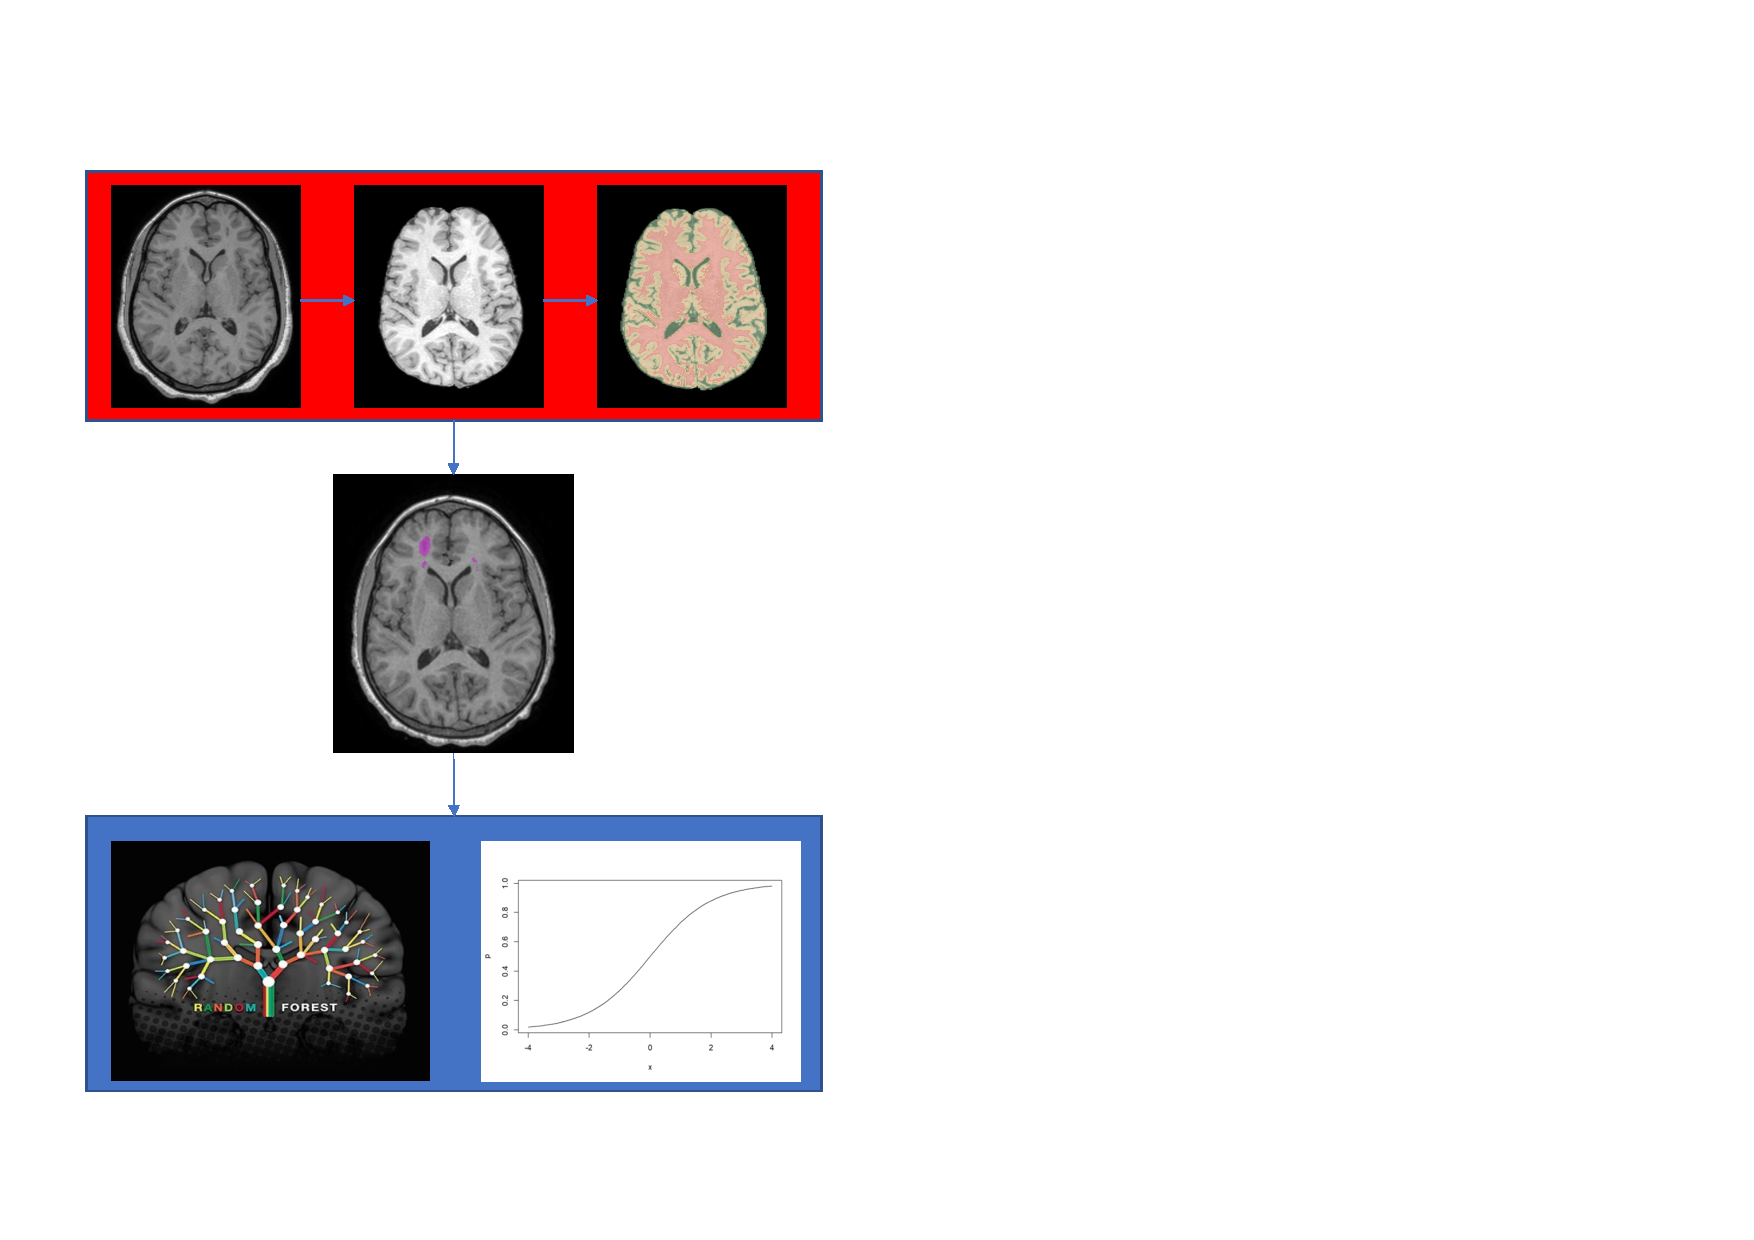
\includegraphics[scale=0.4]{./IMG/Flowchart_img.pdf}
			\end{figure}
		\end{column}
	\end{columns}
			
	\end{frame}
\end{document}

	
	\documentclass[]{standalone}

\begin{document}
	\begin{frame}{Pre-Processing}{Brain Extraction, Normalization, Tissue Segmentation}
		\vspace{-39pt}
		\begin{figure}[h!]
					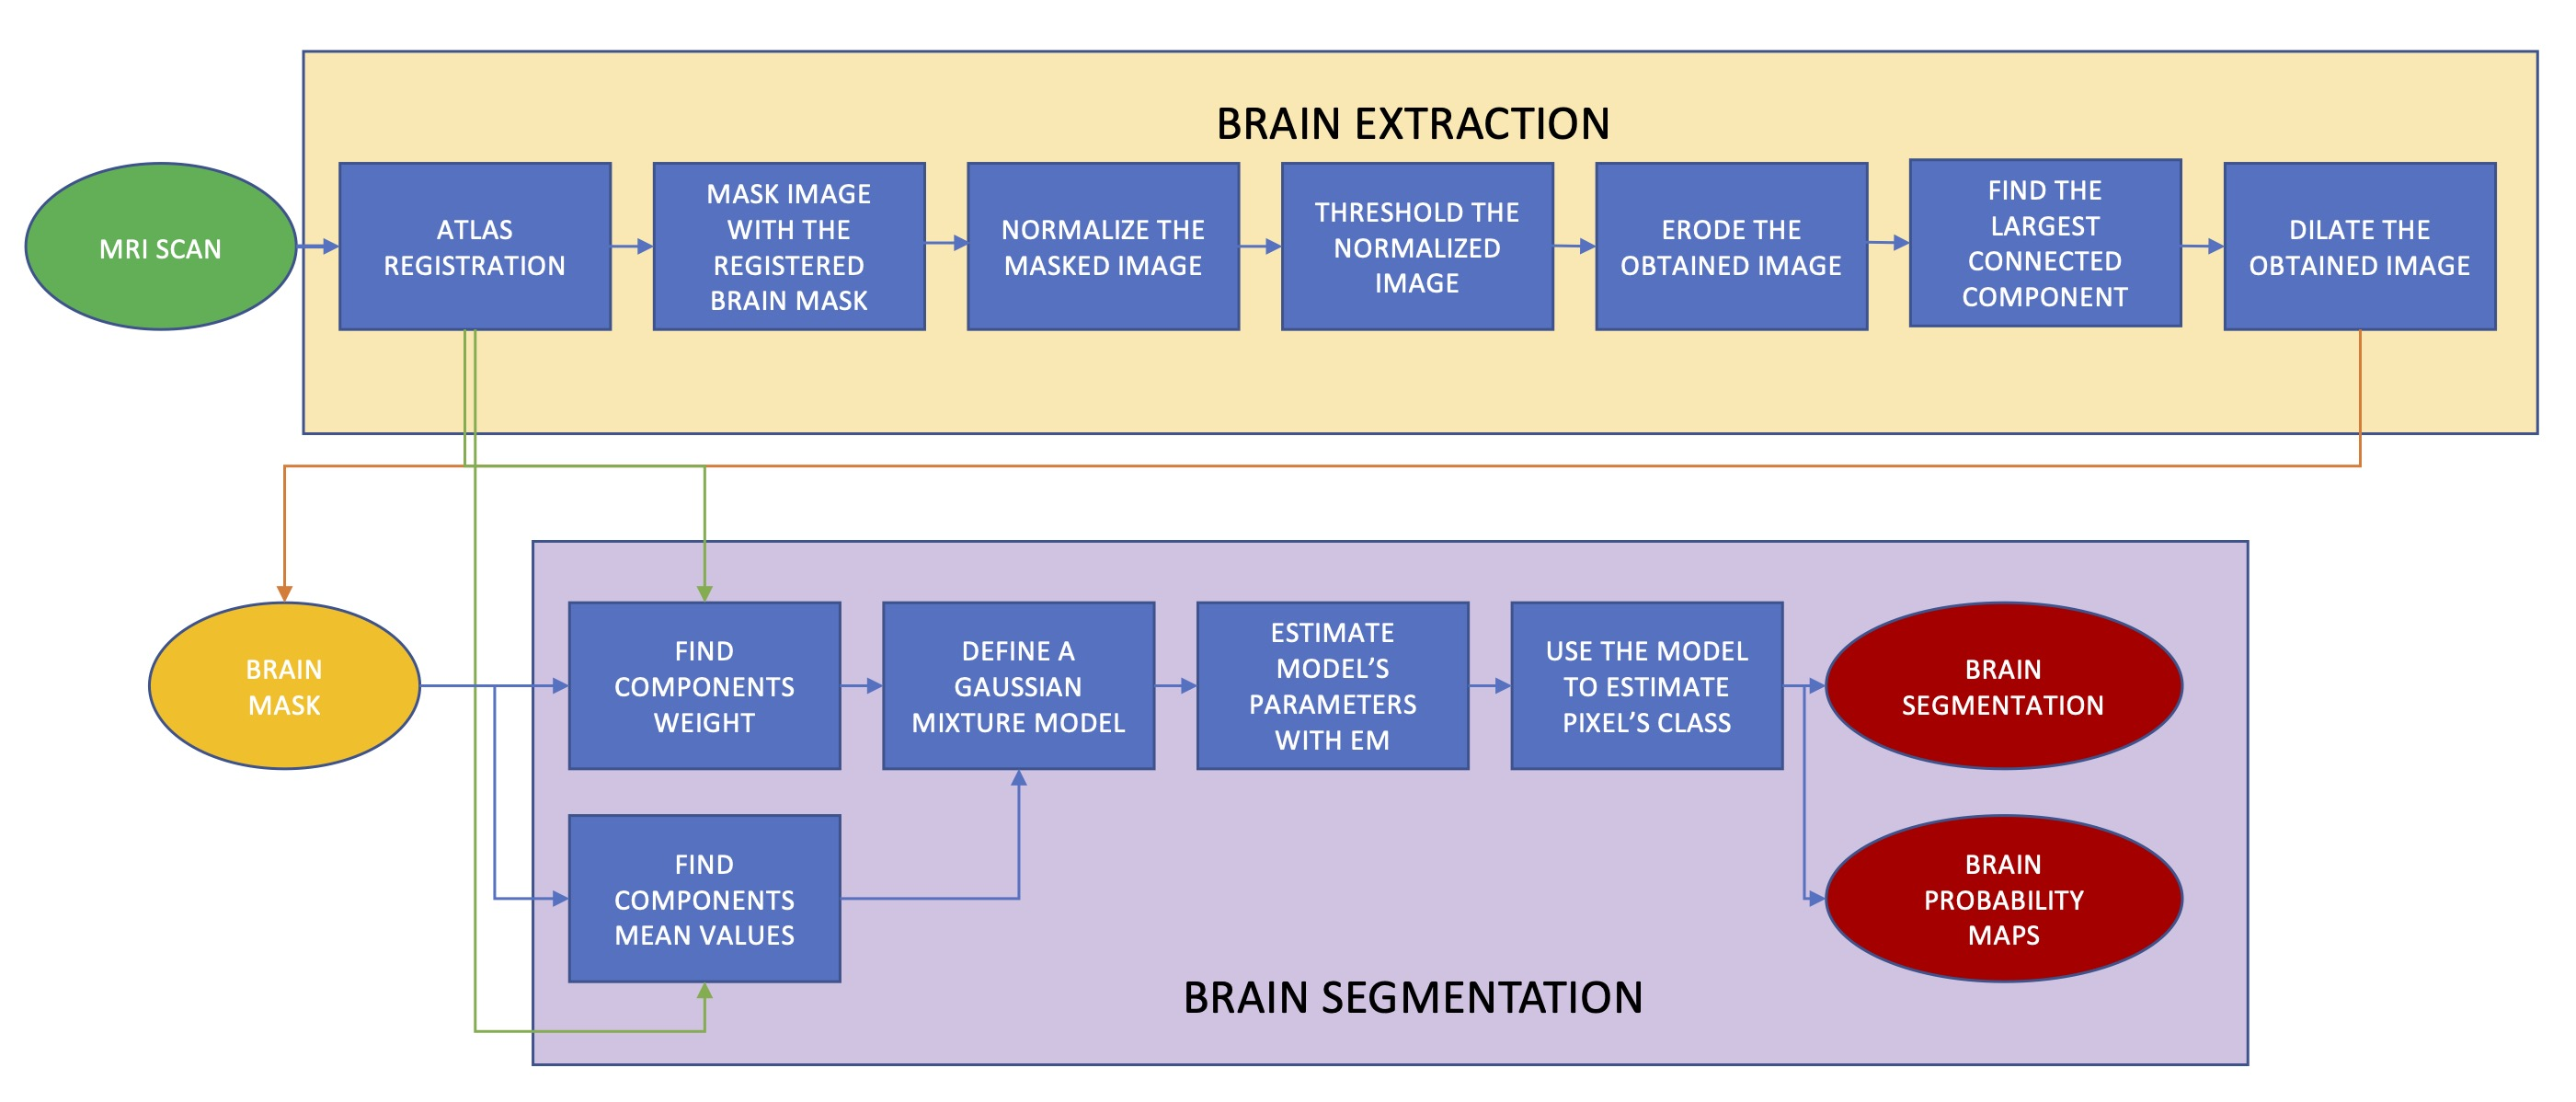
\includegraphics[scale = 0.1, width=\textwidth]{./IMG/FLOWCHART_PRE.jpg}
				\end{figure}
				
		\vspace{-12pt}
		\begin{columns}
			\begin{column}{0.5\textwidth}
			\small
				The Pre-Processing pipeline use an already segmented atlas: ICBM MNI 152 was used.
				
			\end{column}
			\begin{column}{0.5\textwidth}
				\begin{figure}[h!]
				\centering
					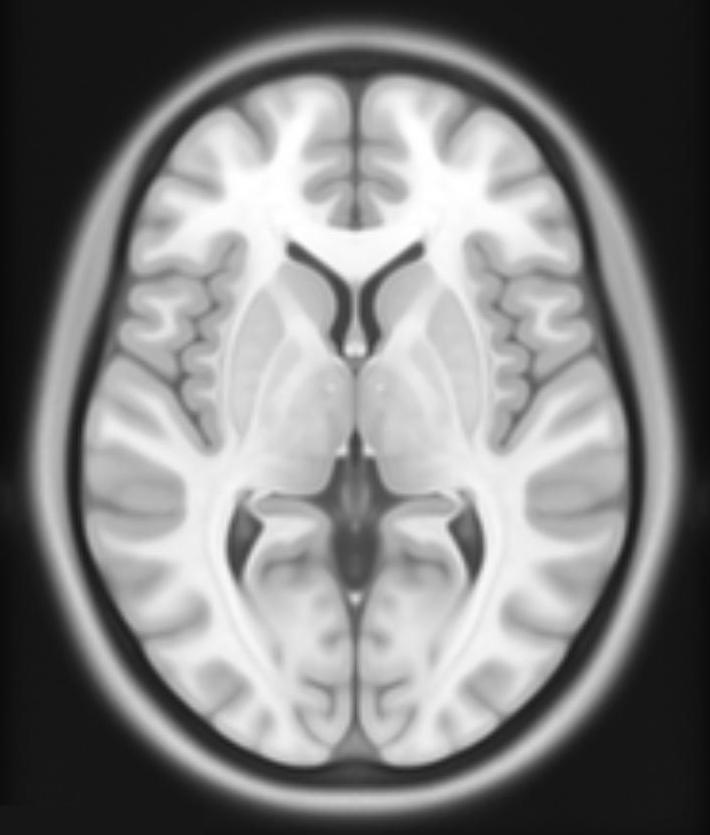
\includegraphics[scale = 0.07]{./IMG/atlas.jpg}
				\end{figure}
				
			\end{column}
		\end{columns}
	\end{frame}
\end{document}

	
	\documentclass[]{standalone}

\begin{document}
	\begin{frame}{Brain Extraction}{Atlas registration, Brain normalization and Skull Stripping}
	
	\vspace{-25pt}
		\begin{columns}
			\begin{column}{0.45\textwidth}
				\begin{itemize}
				\item Atlas Registration;
				\item Normalization;
				\item Thresholding;
				\item Find the Largest Connected Component.
				\end{itemize}
			\end{column}
			\begin{column}{0.55\textwidth}
			\begin{figure}[h!]
			\centering
			\vspace{-6pt}
				\begin{subfigure}{0.45\textwidth}
					\centering
					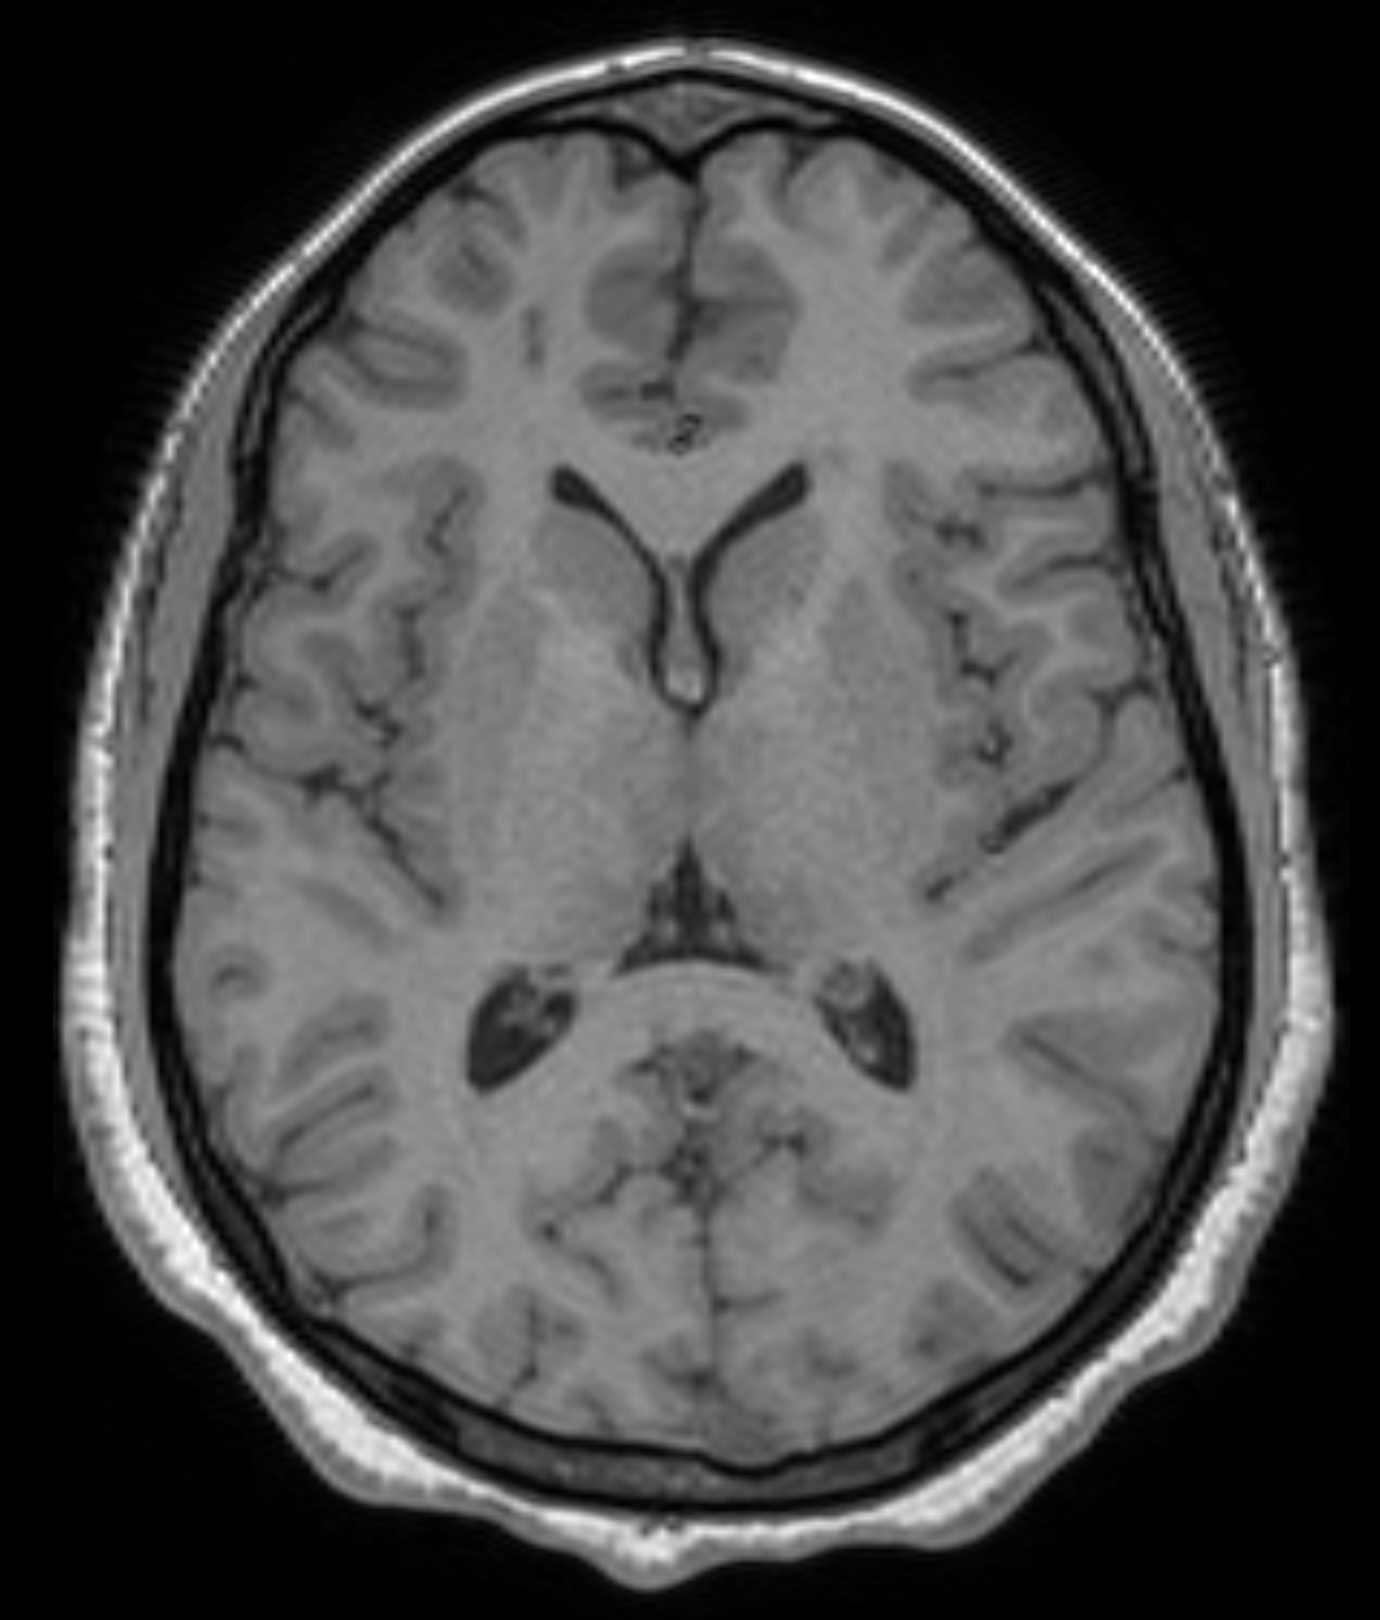
\includegraphics[scale=0.05]{./IMG/T1.jpg}
				\end{subfigure}
				\hfill
				\begin{subfigure}{0.45\textwidth}
					\centering
					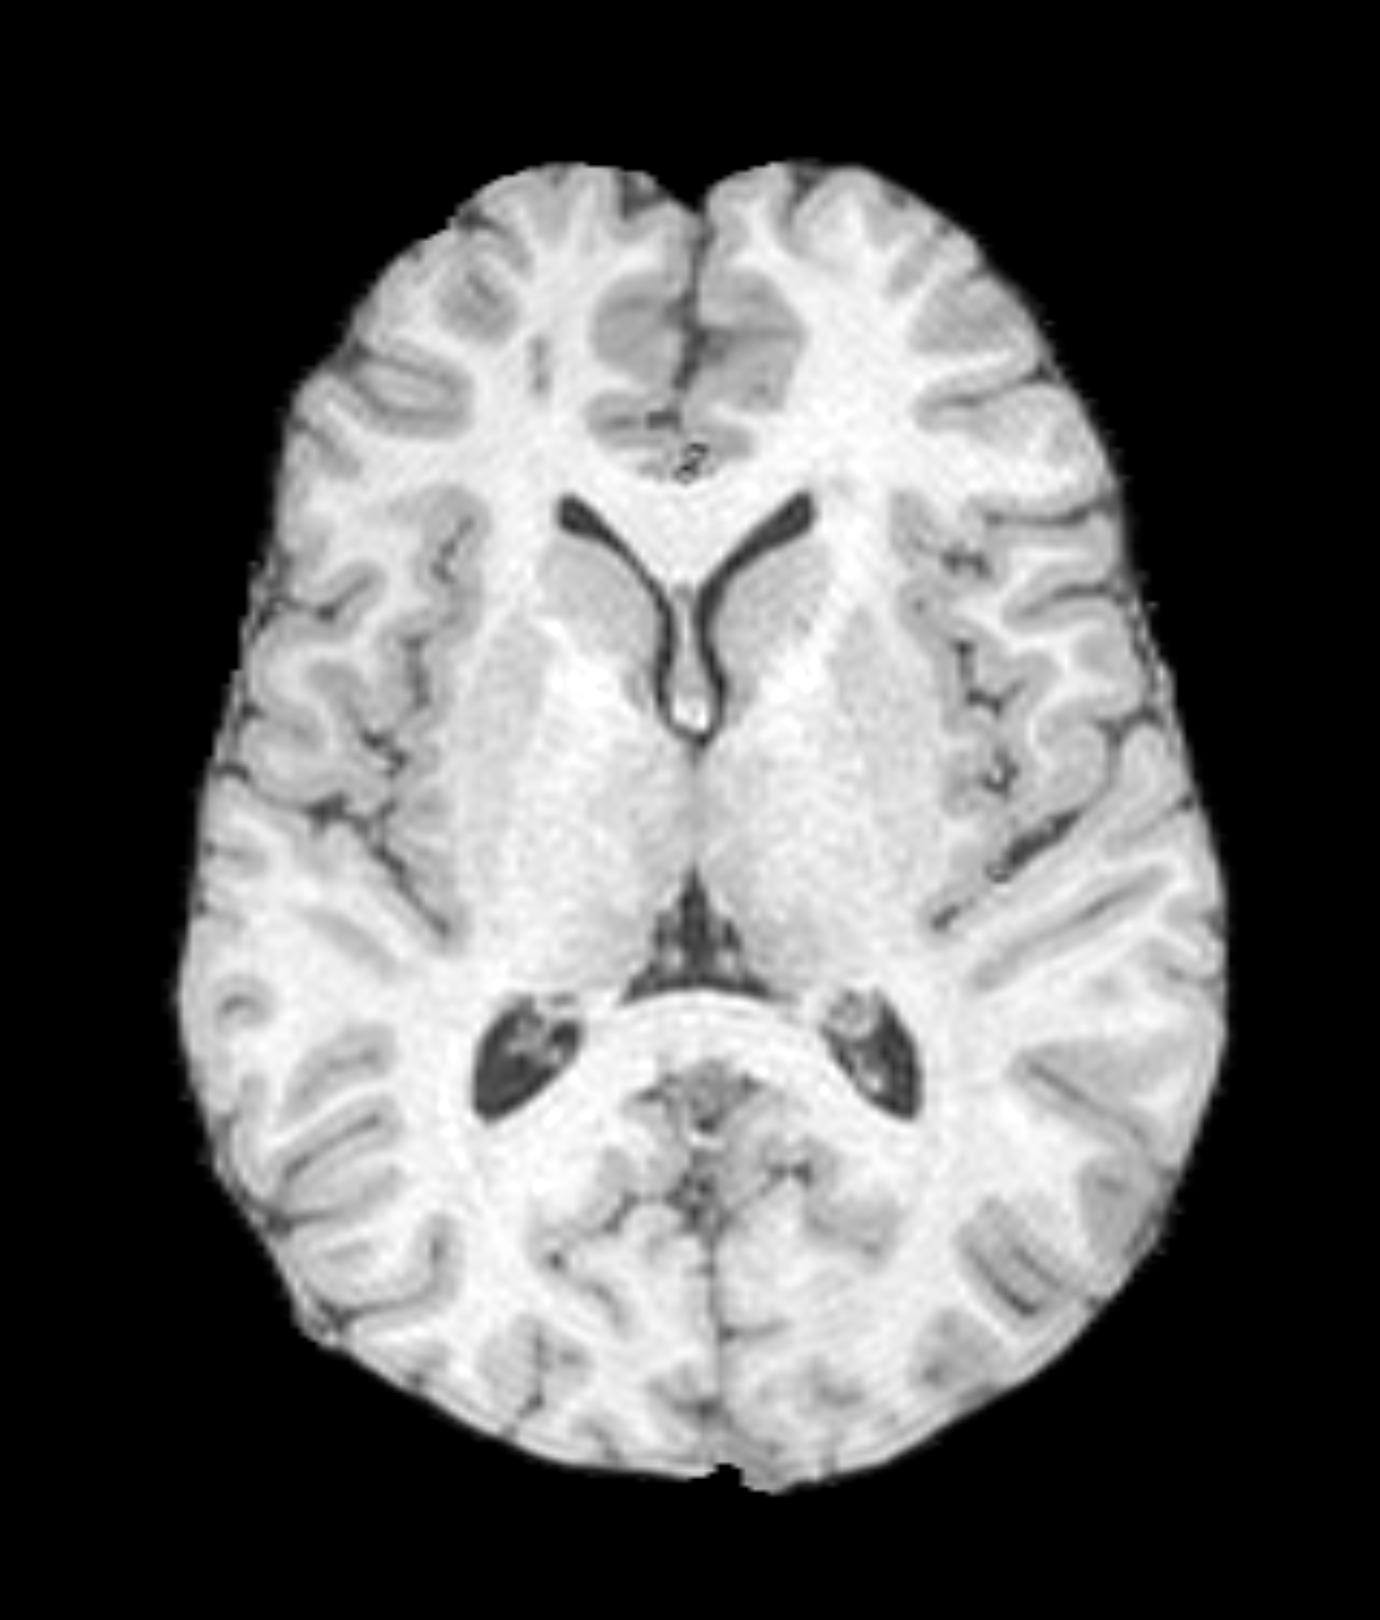
\includegraphics[scale=0.05]{./IMG/brain.jpg}
				\end{subfigure}
				\begin{subfigure}{0.99\textwidth}
					\centering
					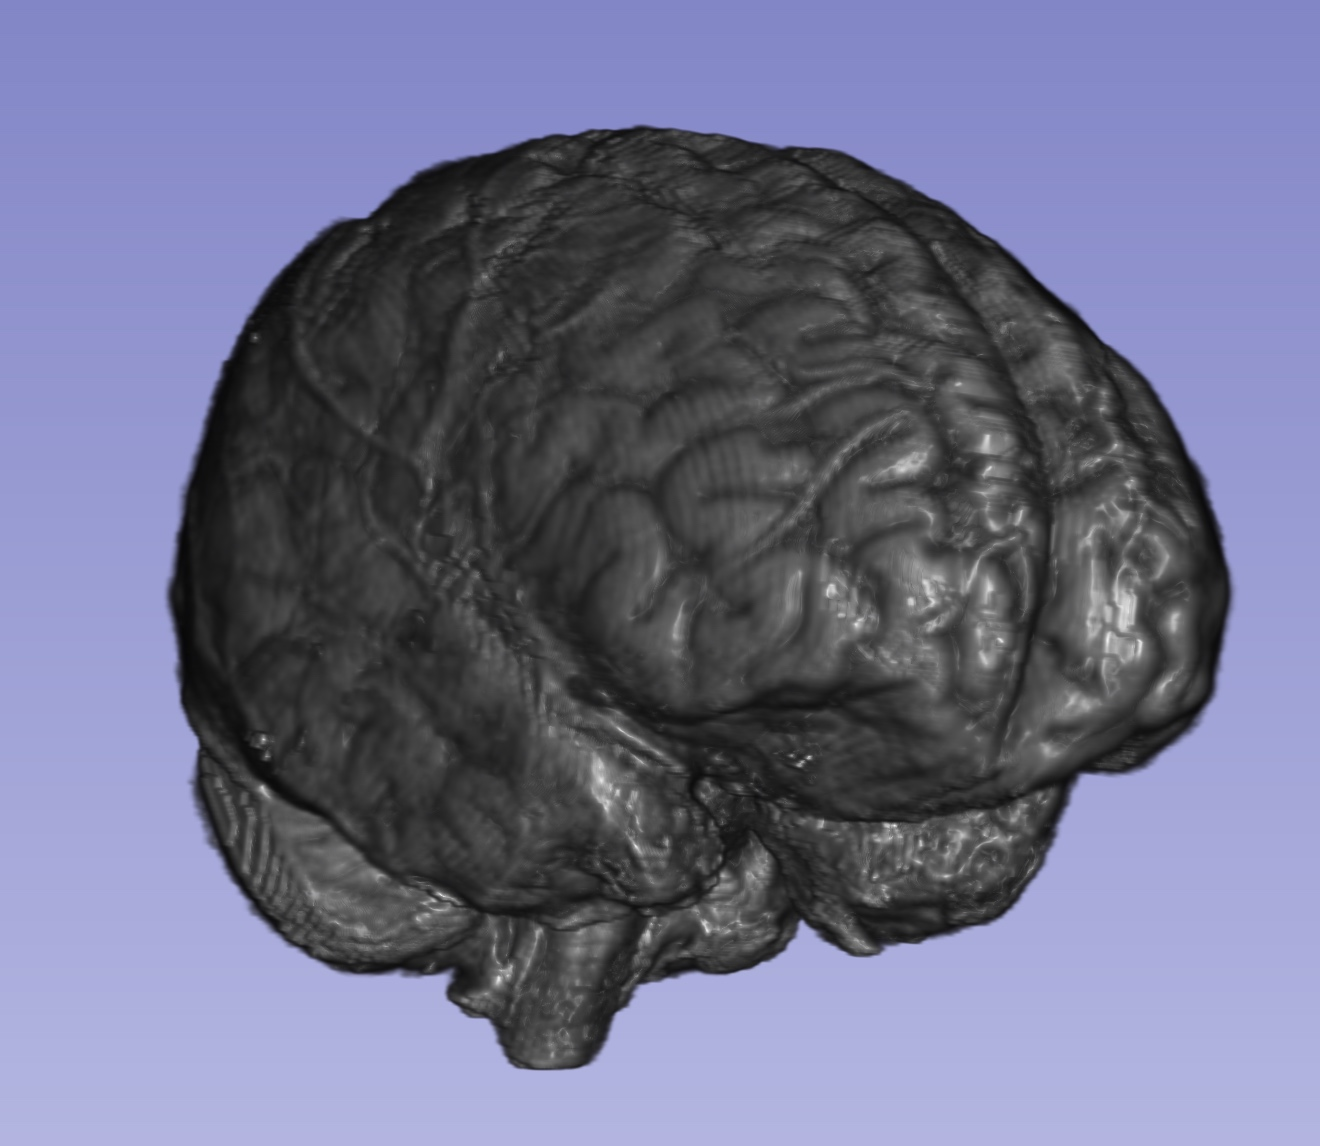
\includegraphics[scale=0.1]{./IMG/3Dbrain.jpg}
				\end{subfigure}
			\end{figure}
			\end{column}
		\end{columns}
	\end{frame}
\end{document}

	
	\documentclass[]{standalone}

\begin{document}
	\begin{frame}{Tissue Segmentation}{A Gaussian Mixture model approach.}
	
	\vspace{-25pt}
		\begin{columns}
			\begin{column}{0.60\textwidth}
			\small
				\begin{itemize}
				\item \textbf{Find Tissues Mean Values and Weights:} Starting from the atlas' partial volume maps compute the mean pixel value and the the fraction of pixels belonging to each tissue;
				\item \textbf{Define a Gaussian Mixture Model:} A mixture of three Gaussian distributions is defined starting from the parameters found;
				\item \textbf{Expectation Maximization:} An expectation maximization algorithm finds the best parameters of the Gaussian mixture model;
				\item \textbf{Classification:} Each pixel is classified.
				\end{itemize}
			\end{column}
			\begin{column}{0.40\textwidth}
			\begin{figure}[h!]
			\centering
			\vspace{-6pt}

				\begin{subfigure}{0.4\textwidth}
					\centering
					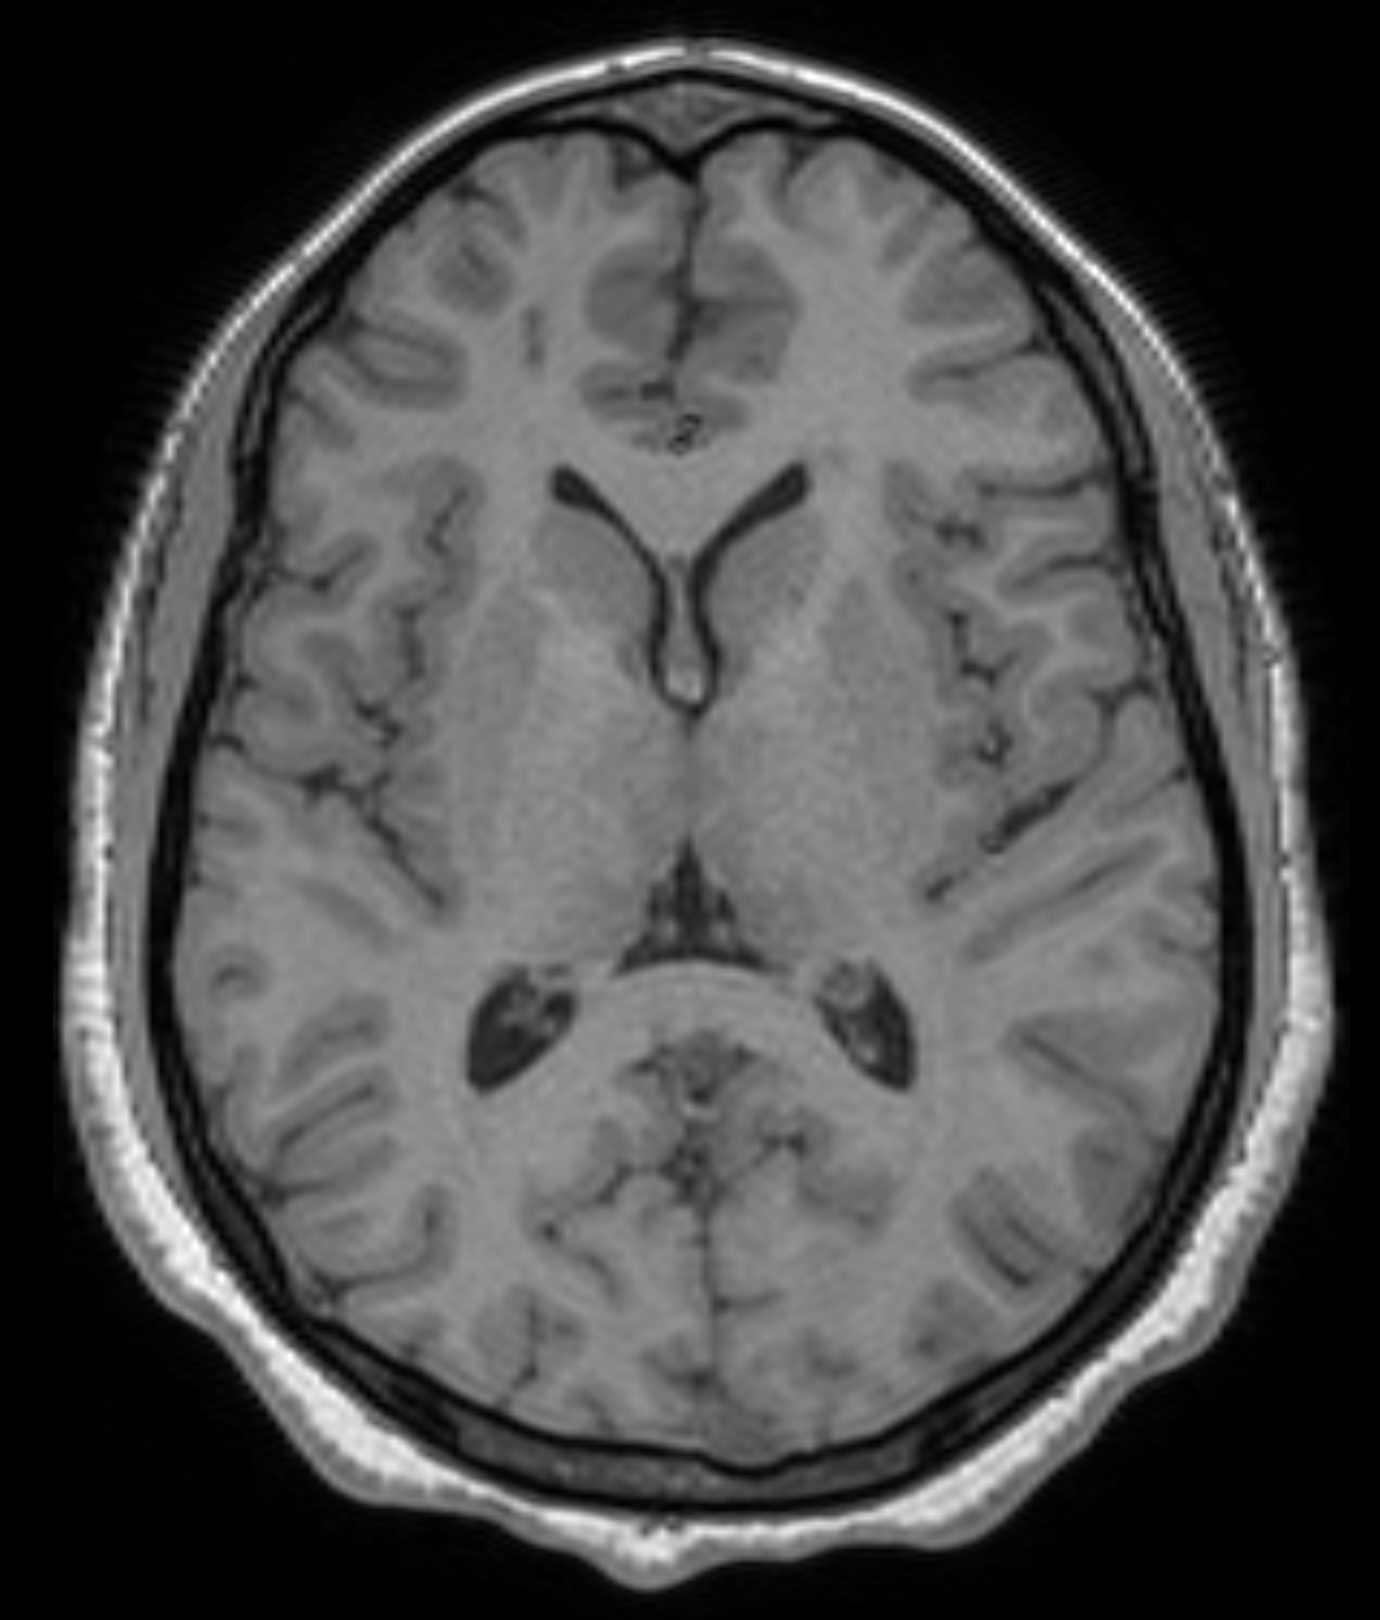
\includegraphics[scale=0.05]{./IMG/T1.jpg}
				\end{subfigure}
				\hspace{10pt}
				\begin{subfigure}{0.4\textwidth}
					\centering
					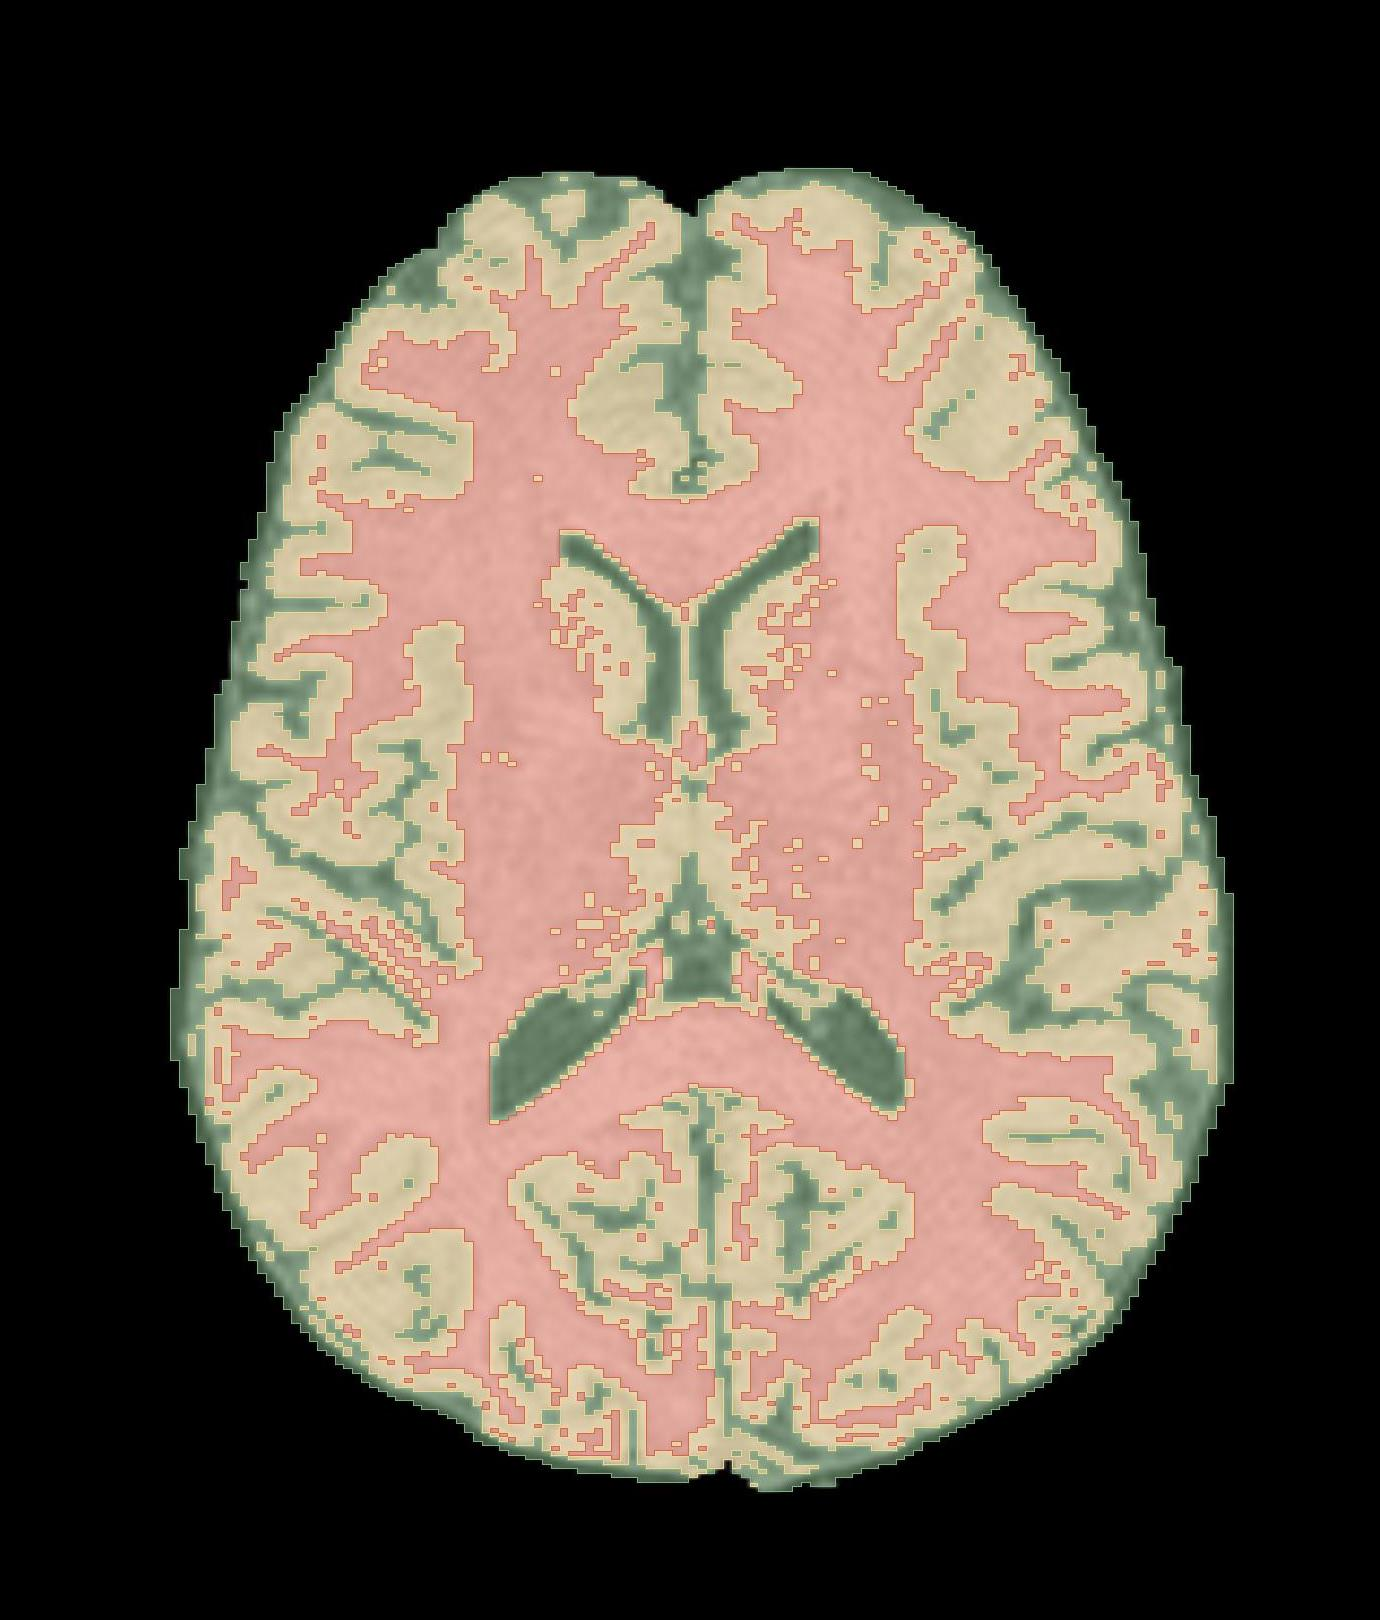
\includegraphics[scale=0.05]{./IMG/segmented_axial.jpg}
				\end{subfigure}

				\begin{subfigure}{0.4\textwidth}
					\centering
					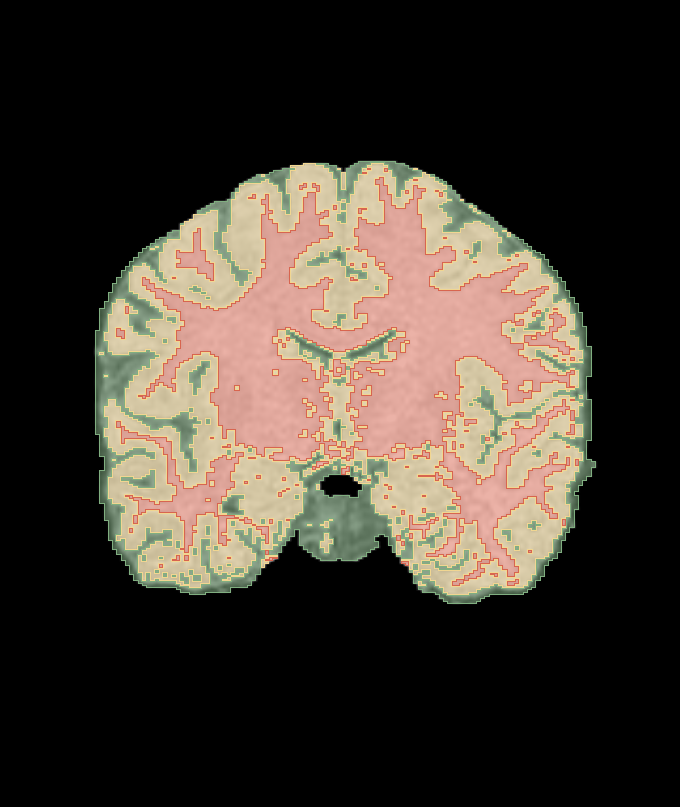
\includegraphics[scale=0.102]{./IMG/segmented_frontal.png}
				\end{subfigure}
				\hspace{10pt}
				\begin{subfigure}{0.4\textwidth}
					\centering
					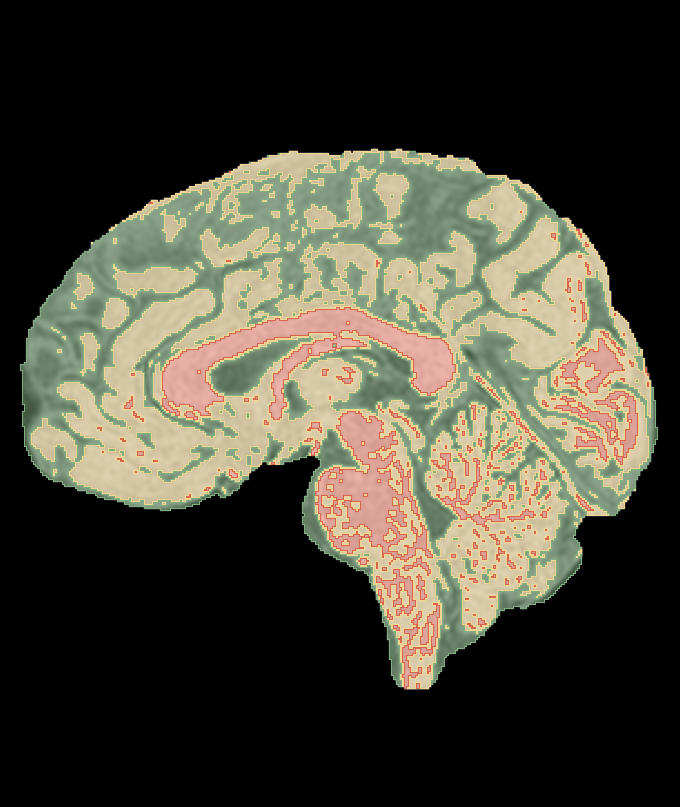
\includegraphics[scale=0.102]{./IMG/segmented_lateral.png}
				\end{subfigure}
				\hspace{10pt}
			\end{figure}
			\end{column}
		\end{columns}
	\end{frame}
\end{document}

	
	\documentclass[]{standalone}

\begin{document}
	\begin{frame}{Post-Processing}{Removals of the False Positives.}
	\vspace{-20pt}
		\begin{figure}[h!]
			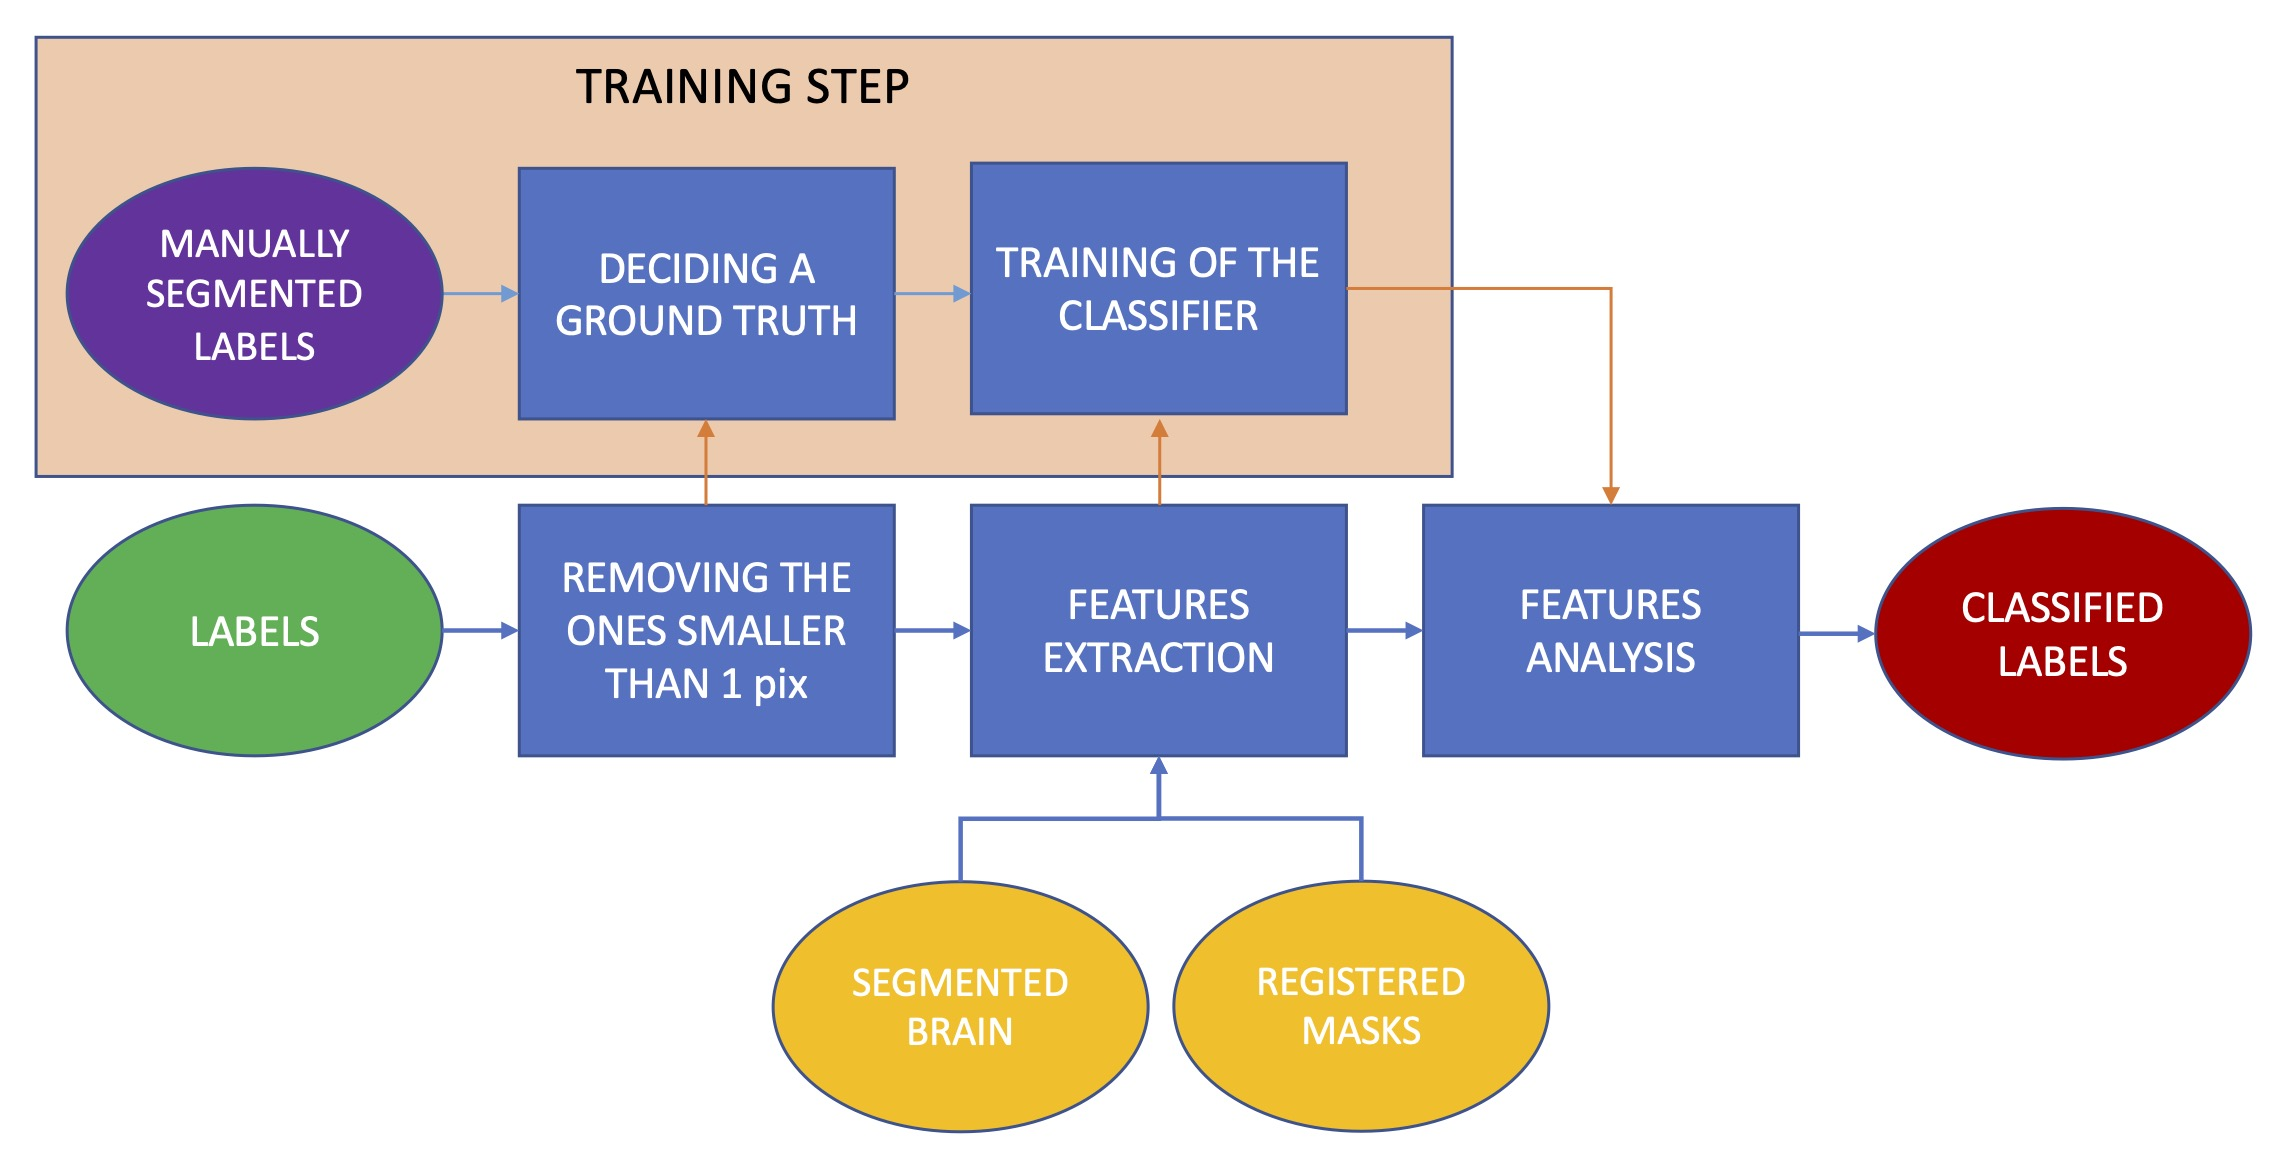
\includegraphics[width = \textwidth]{./IMG/FLOWCHART_POST.jpg}
		\end{figure}

	\end{frame}
\end{document}

	
	\documentclass[]{standalone}

\begin{document}
	\begin{frame}{Features Extraction}{}
	
	
		\begin{columns}
			\begin{column}{0.45\textwidth}
			\small
			Seven different features were extracted for each segmented lesion:
				\begin{itemize}
				\item Lesion probability;
				\item Label's volume;
				\item Overlapping with boundary region mask;
				\item Overlapping with exclusion region mask;
				\item Probability to belong to each tissue.
				\end{itemize}
			\end{column}
			\begin{column}{0.60\textwidth}
			
			\begin{alertblock}{}
				The boundary and exclusion masks manually segmented on the MNI 152 atlas by expert clinicians.
			\end{alertblock}
			
			\hspace{-10pt}
			\begin{figure}[h!]
			\centering
			\vspace{-20pt}

				\begin{subfigure}{0.4\textwidth}
					\centering
					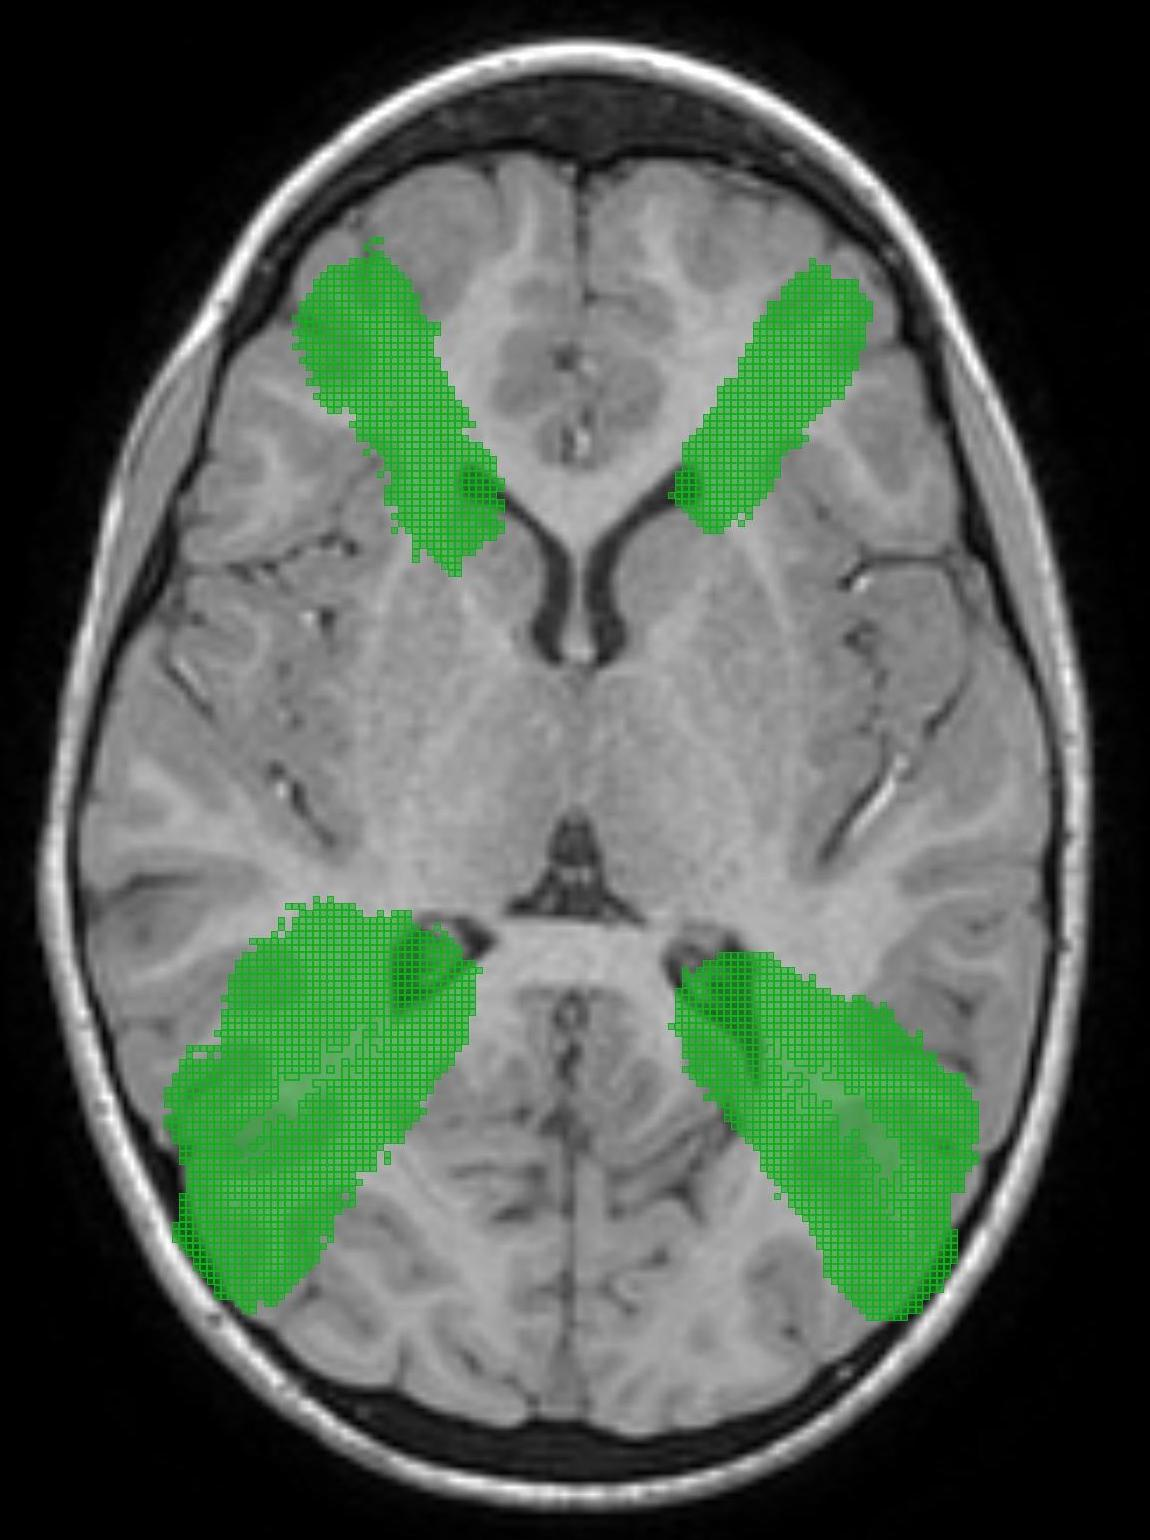
\includegraphics[scale=0.07]{./IMG/boundary.jpg}
					\caption*{Boundary.}
				\end{subfigure}
				\hspace{15pt}
				\begin{subfigure}{0.4\textwidth}
					\centering
					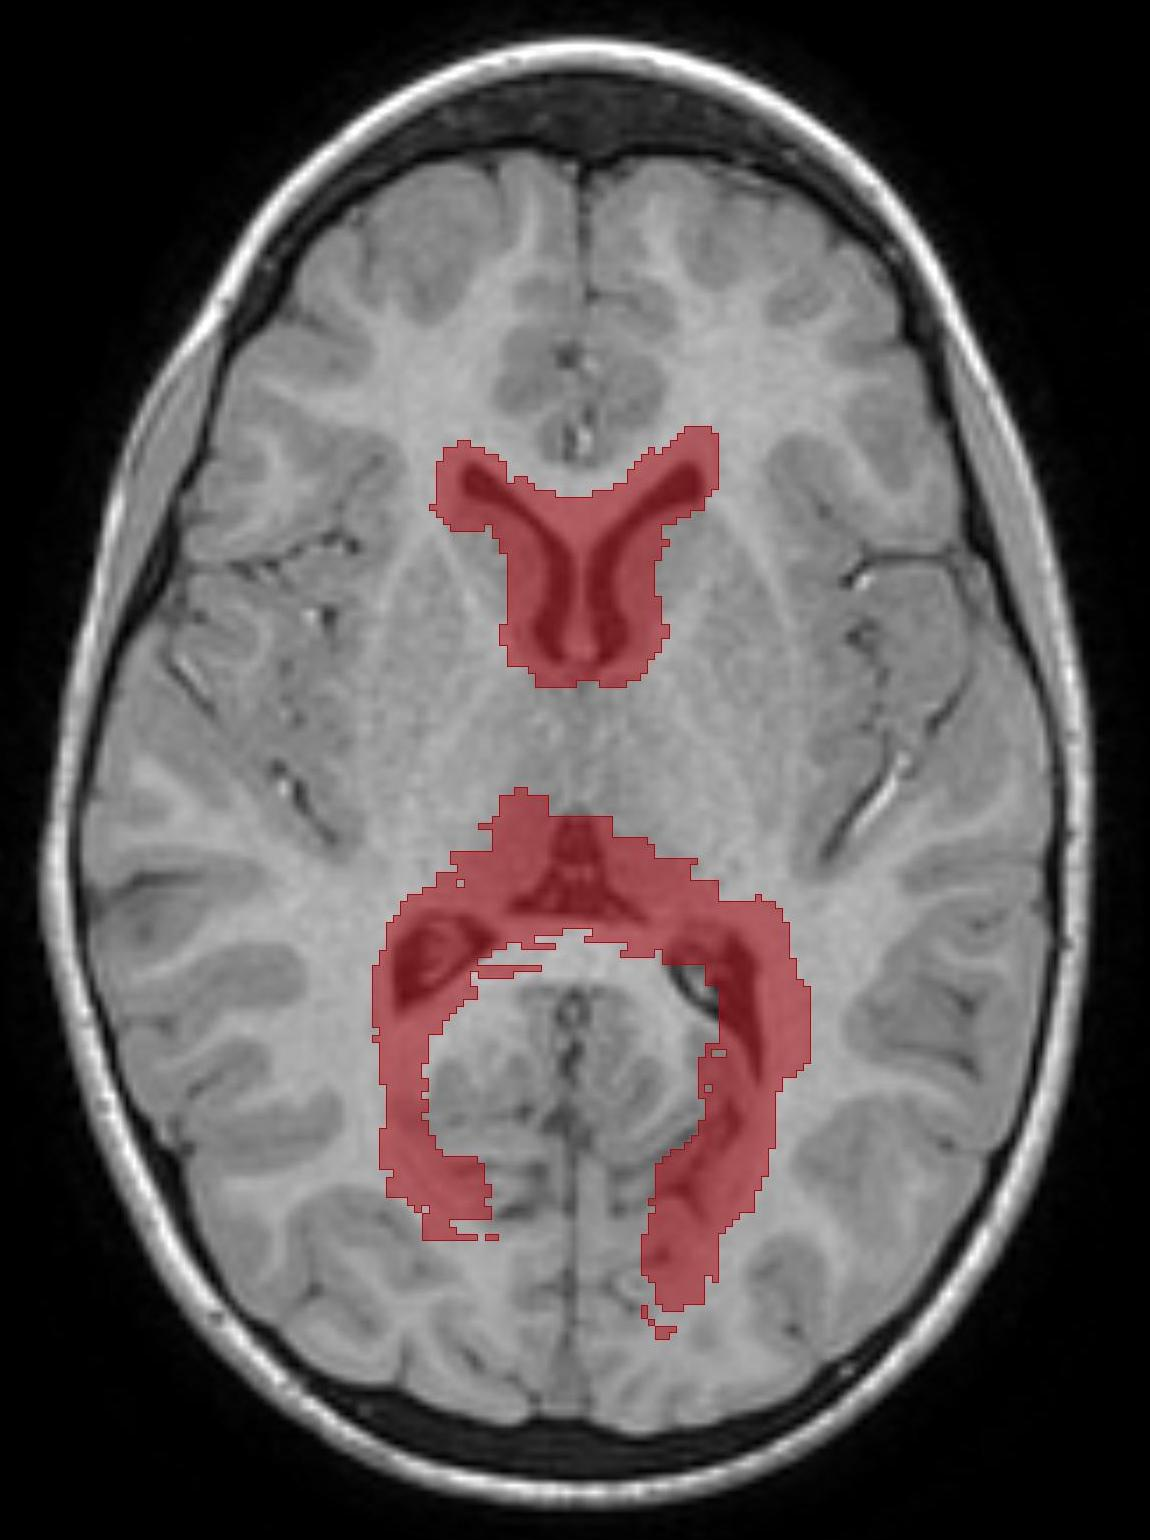
\includegraphics[scale=0.07]{./IMG/exclude.jpg}
					\caption*{Exclusion.}
				\end{subfigure}
			\end{figure}
			\end{column}
		\end{columns}
	\end{frame}
\end{document}

	
	\documentclass[]{standalone}

\begin{document}
	\begin{frame}{Training}{Classifiers, Data Sets, Data Processing}
	\vspace{-25pt}
	\begin{columns}
		\begin{column}{0.33\textwidth}
		\begin{block}{Classifiers}
		Three different classifiers were implemented:
		\begin{itemize}
			\item Decision Tree;
			\item Logistic Regression;
			\item Random Forest.
		\end{itemize}
		\end{block}
		\end{column}
		
		\begin{column}{0.33\textwidth}
		\begin{exampleblock}{Data Sets}
		The data set was previously divided in:
		\begin{itemize}
			\item 51 scans: Training;
			\item 6 scans: Test.
		\end{itemize}
		The division kept in account heterogeneity for:
		\begin{itemize}
			\item Center of provenience;
			\item Scan's resolution;
			\item Presence of lesions.
		\end{itemize}
		\end{exampleblock}
		\end{column}
		
		\begin{column}{0.33\textwidth}
		\begin{alertblock}{Data Processing}
		The training data set was highly unbalanced: $3.7\%$ considered true.
		\begin{itemize}
			\item SMOTE resampling;
			\item Random undersampling;
			\item Robust Features Scaler.
		\end{itemize}
		\end{alertblock}
		\end{column}
		
		
	\end{columns}
	\end{frame}
\end{document}

	
	\documentclass[]{standalone}

\begin{document}
	\begin{frame}{Results}{\textbf{Pre}-Processing}
	\vspace{-28pt}
	
	\begin{columns}
		\begin{column}{0.35\textwidth}
		\begin{itemize}
	
		\item Comparison with masks obtained with FSL;
		\item Computed metric: Dice Similarity Coefficient (DSC).
	\end{itemize}
	
		\begin{equation*}
			    DSC = 2\frac{|X \cap Y |}{|X| + |Y|}
		\end{equation*}
		\end{column}
		
		\begin{column}{0.65\textwidth}
		\begin{block}{Dice Similarity Coefficient}
		\begin{table}[h!]
			\centering
			\small
			\setlength{\tabcolsep}{3pt}
			\begin{tabular}{c|cccc}
					    & \textbf{Mean} & \textbf{Std. Dev.} & \textbf{Median} & \textbf{IQR} \\ \hline
			\textbf{Brain Mask} & 0.87          & 0.12               & 0.93            & 0.11         \\
			\textbf{WM}         & 0.78          & 0.19               & 0.83            & 0.19         \\
			\textbf{GM}         & 0.67          & 0.30               & 0.80            & 0.28         \\
			\textbf{CSF}        & 0.66          & 0.24               & 0.79            & 0.22        
			\end{tabular}
			\end{table}
			\vspace{-10pt}
		\end{block}
			\vspace{-5pt}
			\begin{figure}[h!]
			\tiny
			\centering
				\begin{subfigure}{0.3\textwidth}
					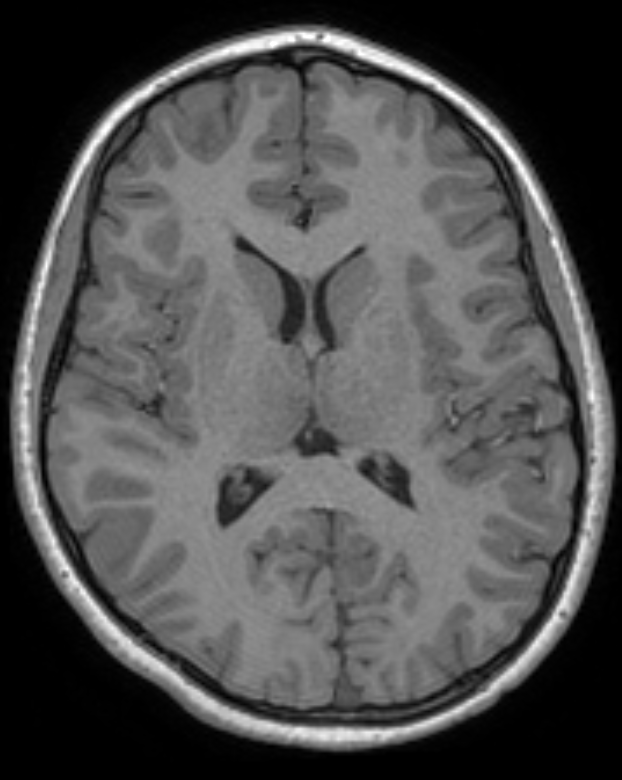
\includegraphics[scale=0.11]{./IMG/T1W48.png}
					\caption*{\tiny T1W }
				\end{subfigure}
				\hfill
				\begin{subfigure}{0.3\textwidth}
					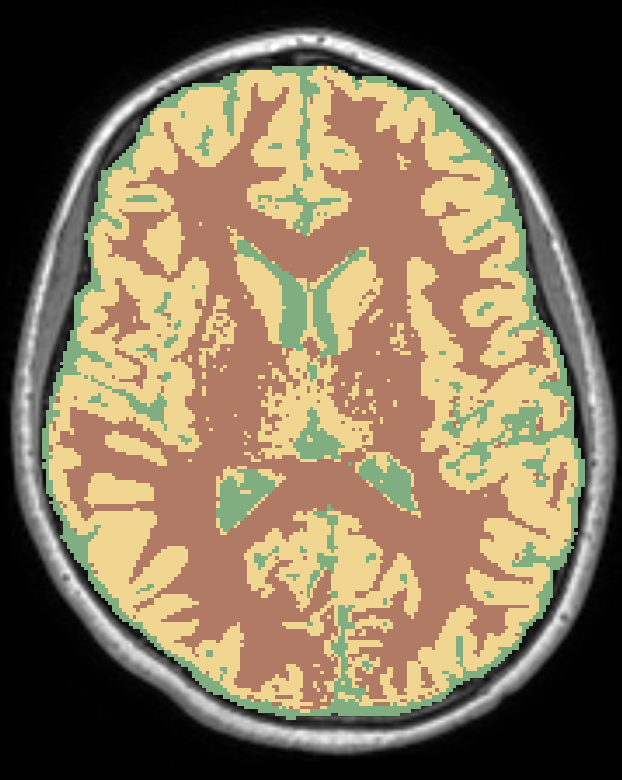
\includegraphics[scale=0.11]{./IMG/FSL_SEG48.png}
					\caption*{\tiny FSL}
				\end{subfigure}
				\hfill
				\begin{subfigure}{0.3\textwidth}
					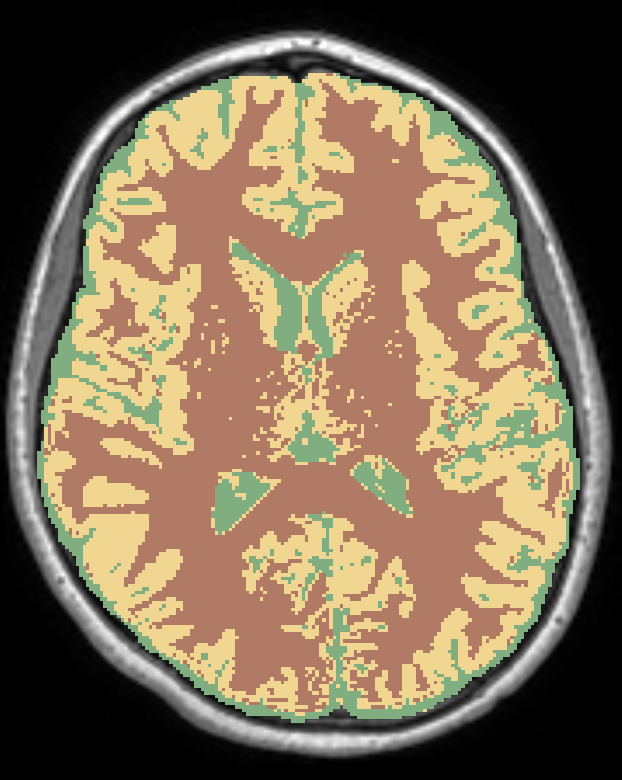
\includegraphics[scale=0.11]{./IMG/SEG48.png}
					\caption*{\tiny Proposed}
				\end{subfigure}
			\end{figure}
		\end{column}
	\end{columns}
	
	\end{frame}
\end{document}

	
	\documentclass[]{standalone}

\begin{document}
	\begin{frame}{Reults}{\textbf{Pre}-Processing}
	\vspace{-25pt}
	Dice coefficient measures overlapping between two images.
	\begin{columns}
		\begin{column}{0.45\textwidth}
		\begin{figure}[h!]
		\footnotesize
		\centering
			\begin{subfigure}[h!]{0.49\textwidth}
			\hfill
			     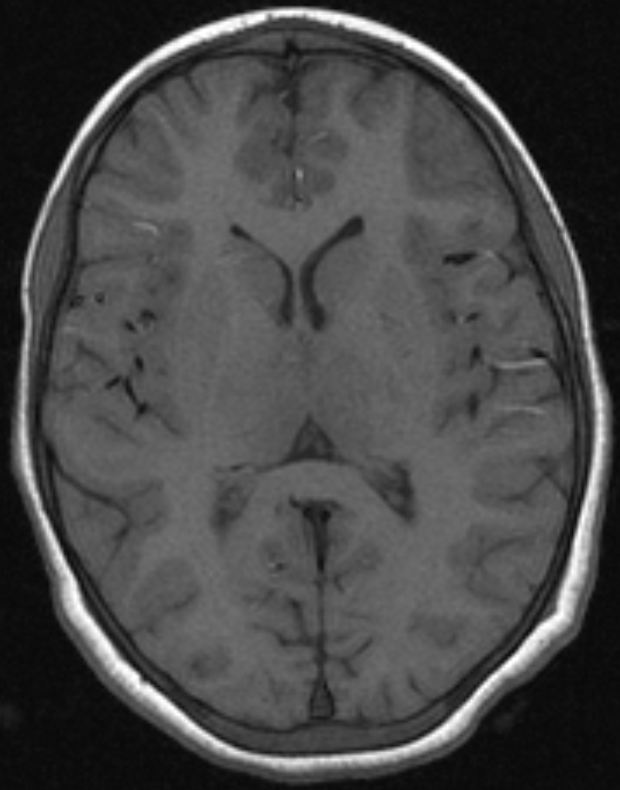
\includegraphics[scale=0.11]{./IMG/T1W0.png}
			     \caption*{Original Scan} 
			\end{subfigure}
			\hfill
			\begin{subfigure}[h!]{0.49\textwidth}
			     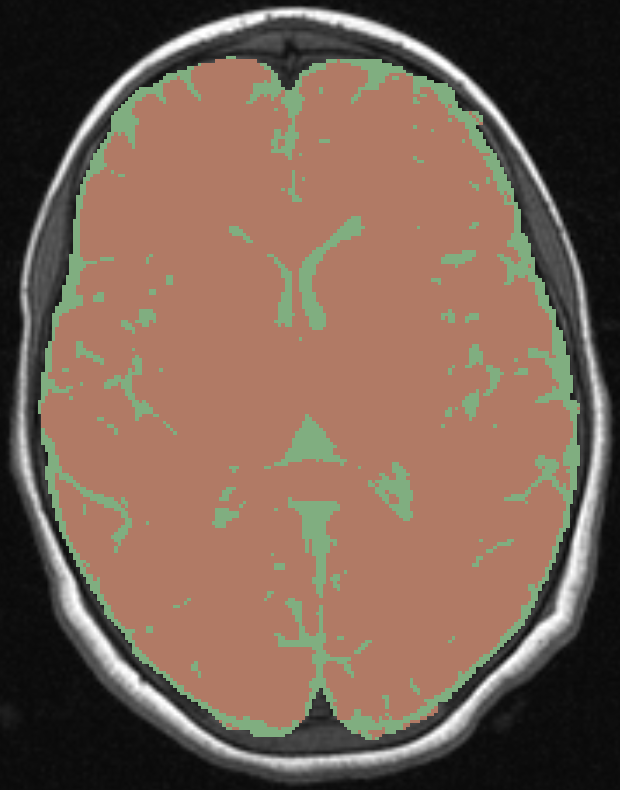
\includegraphics[scale=0.11]{./IMG/SEG0.png}
			     \caption*{Segmentation}
			\end{subfigure}
			\caption*{Pipeline Fault}
		\end{figure}
		\end{column}
		
		\begin{column}{0.55\textwidth}
			\begin{figure}[h!]
			\footnotesize
			\centering
				\begin{subfigure}[h!]{0.32\textwidth}
				     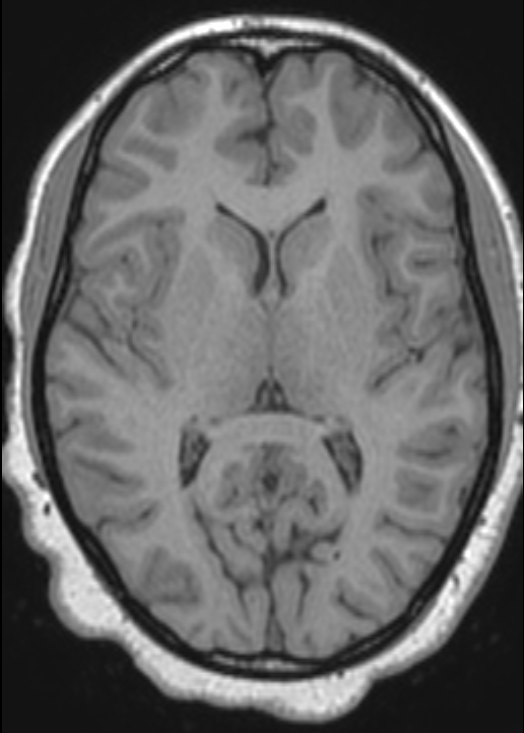
\includegraphics[scale=0.1085]{./IMG/T1W54_2.png}
				     \caption*{Original Scan} 
				\end{subfigure}
				\hfill
				\begin{subfigure}[h!]{0.32\textwidth}
				     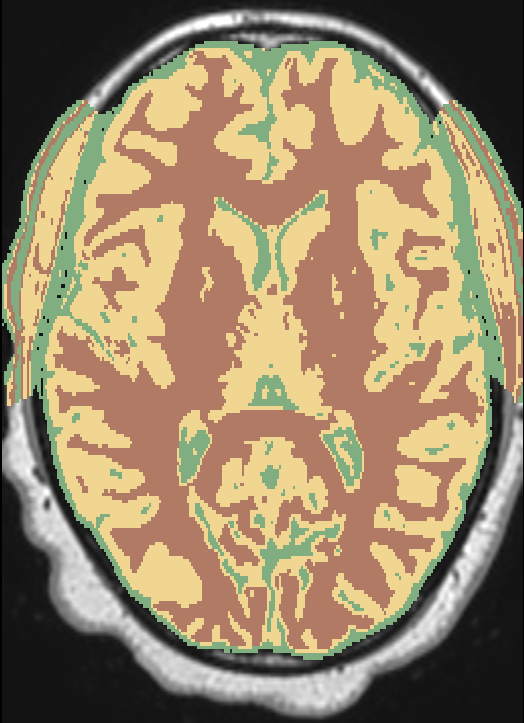
\includegraphics[scale=0.11]{./IMG/FSL_SEG54.png}
				     \caption*{FSL}
				\end{subfigure}
				\hfill
				\begin{subfigure}[h!]{0.32\textwidth}
				     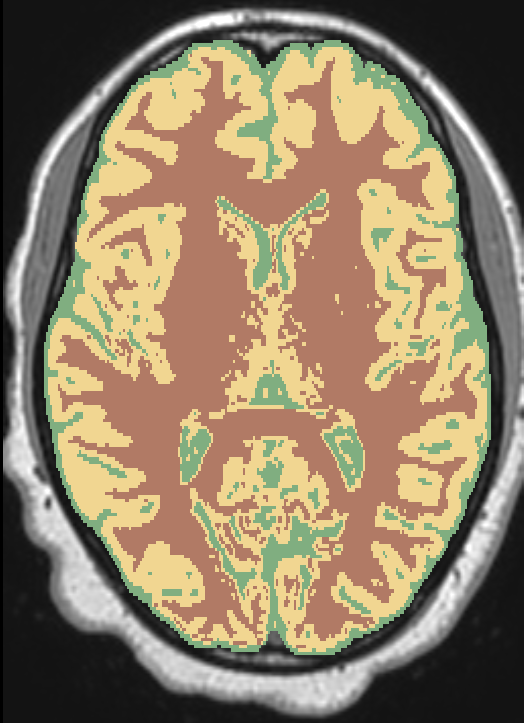
\includegraphics[scale=0.11]{./IMG/SEG54.png}
				     \caption*{Pipeline}
				\end{subfigure}
				\caption*{FSL Fault}
			\end{figure}
		\end{column}
	\end{columns}
	\end{frame}
\end{document}

	
	\documentclass[]{standalone}

\begin{document}
	\begin{frame}{Results}{\textbf{Post}-Processing}
	\vspace{-28pt}
	\begin{block}{Classifiers Performances}
	\begin{table}[h!]
		\centering
		\setlength{\tabcolsep}{2pt}
		\small
		\begin{tabular}{c|ccccc}
		 & \textbf{Bal. Acc.} & \textbf{AUC ROC} & \textbf{AUC PR} & \textbf{Precision} & \textbf{Recall} \\ \hline
		\textbf{Decision Tree}       & 0.74 & 0.81 & 0.45 & 0.38 & 0.96 \\
		\textbf{Logistic regression} & 0.68 & 0.83 & 0.61 & 0.32 & 0.96 \\
		\textbf{Random Forest}       & \textbf{0.74} & \textbf{0.90} & \textbf{0.74} & \textbf{0.38} & \textbf{0.97}
		\end{tabular}
	\end{table}
	\end{block}
	
	\begin{exampleblock}{Features' Importance}
	\begin{table}[h!]
		\centering
		\footnotesize
		\setlength\tabcolsep{2pt}
		\begin{tabular}{c|ccccccc}
				& \textbf{Prob.}     & \textbf{Size}        & \textbf{Boundary}     & \textbf{Exclusion} & \textbf{WM}       & \textbf{GM}        & \textbf{CSF}       \\ \hline
		\textbf{Dec. Tree} & 0.000 & 0.0133 & 0.032 & 0.034 & 0.659 & 0.042 & 0.098 \\
		\textbf{Log. reg.} & 0.00 & $0.0883$ & 0.236 & -1.50 & $1.07 \times 10^5 $ & $4.58 \times 10^4$ & $7.82 \times 10^3$ \\
		\textbf{Rnd F.} & $0.000$ & $0.146$ & $0.027$ & $0.029$  & $0.615$ & $0.067$ & $0.116$
		\end{tabular}
		\end{table}


	\vspace{-10pt}
	\end{exampleblock}

	\end{frame}
\end{document}

	
	\documentclass[]{standalone}

\begin{document}
	\begin{frame}{Conclusions}{}
	\vspace{-5pt}
	\begin{block}{Pre-Processing}
	\footnotesize
	\begin{itemize}
		\item Fully automated;
		\item Good DSC in a comparison with standard used softwares;
		\item Standardized images provided to U-Net permitting a better SCI segmentation;
		\item The proposed pipeline was presented at the European Hematology Association congress in 2022*.
	\end{itemize}
	\end{block}
	
	\begin{exampleblock}{Post-Processing}
	\footnotesize
	\begin{itemize}
		\item Fully automated;
		\item Improved U-Net results;
		\item Explainable features and classifiers.
	\end{itemize}
	\end{exampleblock}
	
	\vspace{5pt}
	\tiny
	*: HemaSphere 6 (2022), pp. 166–167.
	\end{frame}
\end{document}

	
	
	%%%%%%%%%%% APPENDICI
	\appendix

	
	\documentclass[]{standalone}

\begin{document}
	\begin{frame}{Ground Truth Decision}{Modified Jaccard Score}
	\vspace{-25pt}
	\small
	To decide if a automatically found label is to considered true it was necessary to:
	\begin{itemize}
		\item Define an overlapping metric;
		\item Measure the overlapping of a label with the manually segmented ones;
		\item Decide a threshold.
	\end{itemize}
	
	\begin{block}{Modified Jaccard Score}
		\begin{equation*}
		    score(X) = \frac{|X \cap (Y_1 \cup Y_2 \cup ... \cup Y_n)|}
		    {|X \cup (Y_1 \cup Y_2 \cup ... \cup Y_n)|}
		\end{equation*}
		
		\tiny
		\begin{itemize}
			\item X : automatic segmented label;
			\item $Y_i$ : overlapping manual label;
			\item n : number of overlapping manual labels.
		\end{itemize}
	\end{block}
	\end{frame}
\end{document}

	

\end{document}
